 % uWaterloo Thesis Template for LaTeX 
% Last Updated May 24, 2011 by Stephen Carr, IST Client Services
% FOR ASSISTANCE, please send mail to rt-IST-CSmathsci@ist.uwaterloo.ca
% ADDED THIS LINE FROM THE OTHER SIDE
% Effective October 2006, the University of Waterloo 
% requires electronic thesis submission. See the uWaterloo thesis regulations at
% http://www.grad.uwaterloo.ca/Thesis_Regs/thesistofc.asp.

% DON'T FORGET TO ADD YOUR OWN NAME AND TITLE in the "hyperref" package
% configuration below. THIS INFORMATION GETS EMBEDDED IN THE PDF FINAL PDF DOCUMENT.
% You can view the information if you view Properties of the PDF document.

% Many faculties/departments also require one or more printed
% copies. This template attempts to satisfy both types of output. 
% It is based on the standard "book" document class which provides all necessary 
% sectioning structures and allows multi-part theses.

% DISCLAIMER
% To the best of our knowledge, this template satisfies the current uWaterloo requirements.
% However, it is your responsibility to assure that you have met all 
% requirements of the University and your particular department.
% Many thanks to the feedback from many graduates that assisted the development of this template.

% -----------------------------------------------------------------------

% By default, output is produced that is geared toward generating a PDF 
% version optimized for viewing on an electronic display, including 
% hyperlinks within the PDF.
 
% E.g. to process a thesis called "mythesis.tex" based on this template, run:

% pdflatex mythesis	-- first pass of the pdflatex processor
% bibtex mythesis	-- generates bibliography from .bib data file(s) 
% pdflatex mythesis	-- fixes cross-references, bibliographic references, etc
% pdflatex mythesis	-- fixes cross-references, bibliographic references, etc

% If you use the recommended LaTeX editor, Texmaker, you would open the mythesis.tex
% file, then click the pdflatex button. Then run BibTeX (under the Tools menu).
% Then click the pdflatex button two more times. If you have an index as well,
% you'll need to run MakeIndex from the Tools menu as well, before running pdflatex
% the last two times.

% N.B. The "pdftex" program allows graphics in the following formats to be
% included with the "\includegraphics" command: PNG, PDF, JPEG, TIFF
% Tip 1: Generate your figures and photos in the size you want them to appear
% in your thesis, rather than scaling them with \includegraphics options.
% Tip 2: Any drawings you do should be in scalable vector graphic formats:
% SVG, PNG, WMF, EPS and then converted to PNG or PDF, so they are scalable in
% the final PDF as well.
% Tip 3: Photographs should be cropped and compressed so as not to be too large.

% To create a PDF output that is optimized for double-sided printing: 
%
% 1) comment-out the \documentclass statement in the preamble below, and
% un-comment the second \documentclass line.
%
% 2) change the value assigned below to the boolean variable
% "PrintVersion" from "false" to "true".

% --------------------- Start of Document Preamble -----------------------

% Specify the document class, default style attributes, and page dimensions
% For hyperlinked PDF, suitable for viewing on a computer, use this:
\documentclass[letterpaper,12pt,titlepage,oneside,final]{book}
 
% For PDF, suitable for double-sided printing, change the PrintVersion variable below
% to "true" and use this \documentclass line instead of the one above:
%\documentclass[letterpaper,12pt,titlepage,openright,twoside,final]{book}

% Some LaTeX commands I define for my own nomenclature.
% If you have to, it's better to change nomenclature once here than in a 
% million places throughout your thesis!
\newcommand{\package}[1]{\textbf{#1}} % package names in bold text
\newcommand{\cmmd}[1]{\textbackslash\texttt{#1}} % command name in tt font 
\newcommand{\href}[1]{#1} % does nothing, but defines the command so the
    % print-optimized version will ignore \href tags (redefined by hyperref pkg).
%\newcommand{\texorpdfstring}[2]{#1} % does nothing, but defines the command
% Anything defined here may be redefined by packages added below...

\usepackage{algorithm}
\usepackage{algpseudocode}
\usepackage{pifont}
\usepackage{amsmath}
\usepackage{amssymb}
\usepackage[pdftex]{graphicx}
\usepackage{enumerate}
\usepackage{amsfonts}
\usepackage{url}
\usepackage{amsmath,amsfonts,amssymb,amsthm,epsfig,epstopdf,titling,url,array}
\usepackage[]{units}
\usepackage{xcolor}
\usepackage{fancybox}
\usepackage{tikz}
\usepackage{stmaryrd}
\usepackage{caption}
\usepackage{subcaption}
\theoremstyle{plain}
\newtheorem{thm}{Theorem}[section]
\newtheorem{lem}[thm]{Lemma}
\newtheorem{prop}[thm]{Proposition}
\newtheorem*{cor}{Corollary}


% This package allows if-then-else control structures.
\usepackage{ifthen}
\newboolean{PrintVersion}
\setboolean{PrintVersion}{false} 
% CHANGE THIS VALUE TO "true" as necessary, to improve printed results for hard copies
% by overriding some options of the hyperref package below.

%\usepackage{nomencl} % For a nomenclature (optional; available from ctan.org)
\usepackage{amsmath,amssymb,amstext} % Lots of math symbols and environments
\usepackage[pdftex]{graphicx} % For including graphics N.B. pdftex graphics driver 

% Hyperlinks make it very easy to navigate an electronic document.
% In addition, this is where you should specify the thesis title
% and author as they appear in the properties of the PDF document.
% Use the "hyperref" package 
% N.B. HYPERREF MUST BE THE LAST PACKAGE LOADED; ADD ADDITIONAL PKGS ABOVE
\usepackage[pdftex,letterpaper=true,pagebackref=false]{hyperref} % with basic options
		% N.B. pagebackref=true provides links back from the References to the body text. This can cause trouble for printing.
\hypersetup{
    plainpages=false,       % needed if Roman numbers in frontpages
    pdfpagelabels=true,     % adds page number as label in Acrobat's page count
    bookmarks=true,         % show bookmarks bar?
    unicode=false,          % non-Latin characters in Acrobat’s bookmarks
    pdftoolbar=true,        % show Acrobat’s toolbar?
    pdfmenubar=true,        % show Acrobat’s menu?
    pdffitwindow=false,     % window fit to page when opened
    pdfstartview={FitH},    % fits the width of the page to the window
    pdftitle={uWaterloo\ LaTeX\ Thesis\ Template},    % title: CHANGE THIS TEXT!
%    pdfauthor={Author},    % author: CHANGE THIS TEXT! and uncomment this line
%    pdfsubject={Subject},  % subject: CHANGE THIS TEXT! and uncomment this line
%    pdfkeywords={keyword1} {key2} {key3}, % list of keywords, and uncomment this line if desired
    pdfnewwindow=true,      % links in new window
    colorlinks=true,        % false: boxed links; true: colored links
    linkcolor=blue,         % color of internal links
    citecolor=green,        % color of links to bibliography
    filecolor=magenta,      % color of file links
    urlcolor=cyan           % color of external links
}
\ifthenelse{\boolean{PrintVersion}}{   % for improved print quality, change some hyperref options
\hypersetup{	% override some previously defined hyperref options
%    colorlinks,%
    citecolor=black,%
    filecolor=black,%
    linkcolor=black,%
    urlcolor=black}
}{} % end of ifthenelse (no else)

% Setting up the page margins...
% uWaterloo thesis requirements specify a minimum of 1 inch (72pt) margin at the
% top, bottom, and outside page edges and a 1.125 in. (81pt) gutter
% margin (on binding side). While this is not an issue for electronic
% viewing, a PDF may be printed, and so we have the same page layout for
% both printed and electronic versions, we leave the gutter margin in.
% Set margins to minimum permitted by uWaterloo thesis regulations:
\setlength{\marginparwidth}{0pt} % width of margin notes
% N.B. If margin notes are used, you must adjust \textwidth, \marginparwidth
% and \marginparsep so that the space left between the margin notes and page
% edge is less than 15 mm (0.6 in.)
\setlength{\marginparsep}{0pt} % width of space between body text and margin notes
\setlength{\evensidemargin}{0.125in} % Adds 1/8 in. to binding side of all 
% even-numbered pages when the "twoside" printing option is selected
\setlength{\oddsidemargin}{0.125in} % Adds 1/8 in. to the left of all pages
% when "oneside" printing is selected, and to the left of all odd-numbered
% pages when "twoside" printing is selected
\setlength{\textwidth}{6.375in} % assuming US letter paper (8.5 in. x 11 in.) and 
% side margins as above
\raggedbottom

% The following statement specifies the amount of space between
% paragraphs. Other reasonable specifications are \bigskipamount and \smallskipamount.
\setlength{\parskip}{\medskipamount}

% The following statement controls the line spacing.  The default
% spacing corresponds to good typographic conventions and only slight
% changes (e.g., perhaps "1.2"), if any, should be made.
\renewcommand{\baselinestretch}{1} % this is the default line space setting

% By default, each chapter will start on a recto (right-hand side)
% page.  We also force each section of the front pages to start on 
% a recto page by inserting \cleardoublepage commands.
% In many cases, this will require that the verso page be
% blank and, while it should be counted, a page number should not be
% printed.  The following statements ensure a page number is not
% printed on an otherwise blank verso page.
\let\origdoublepage\cleardoublepage
\newcommand{\clearemptydoublepage}{%
  \clearpage{\pagestyle{empty}\origdoublepage}}
\let\cleardoublepage\clearemptydoublepage

%======================================================================
%   L O G I C A L    D O C U M E N T -- the content of your thesis
%======================================================================
\begin{document}

% For a large document, it is a good idea to divide your thesis
% into several files, each one containing one chapter.
% To illustrate this idea, the "front pages" (i.e., title page,
% declaration, borrowers' page, abstract, acknowledgements,
% dedication, table of contents, list of tables, list of figures,
% nomenclature) are contained within the file "uw-ethesis-frontpgs.tex" which is
% included into the document by the following statement.
%----------------------------------------------------------------------
% FRONT MATERIAL
%----------------------------------------------------------------------
% T I T L E   P A G E
% -------------------
% Last updated May 24, 2011, by Stephen Carr, IST-Client Services
% The title page is counted as page `i' but we need to suppress the
% page number.  We also don't want any headers or footers.
\pagestyle{empty}
\pagenumbering{roman}

% The contents of the title page are specified in the "titlepage"
% environment.
\begin{titlepage}
        \begin{center}
        \vspace*{1.0cm}

        \Huge
        {\bf Approximately Optimum Search Trees in External Memory Models }

        \vspace*{1.0cm}

        \normalsize
        by \\

        \vspace*{1.0cm}

        \Large
        Oliver Grant \\

        \vspace*{3.0cm}

        \normalsize
        A thesis \\
        presented to the University of Waterloo \\ 
        in fulfillment of the \\
        thesis requirement for the degree of \\
        Master of Mathematics \\
        in \\
        Computer Science \\

        \vspace*{2.0cm}

        Waterloo, Ontario, Canada, 2016 \\

        \vspace*{1.0cm}

        \end{center}
\end{titlepage}

% The rest of the front pages should contain no headers and be numbered using Roman numerals starting with `ii'
\pagestyle{plain}
\setcounter{page}{2}

\cleardoublepage % Ends the current page and causes all figures and tables that have so far appeared in the input to be printed.
% In a two-sided printing style, it also makes the next page a right-hand (odd-numbered) page, producing a blank page if necessary.
 


% D E C L A R A T I O N   P A G E
% -------------------------------
  % The following is the sample Delaration Page as provided by the GSO
  % December 13th, 2006.  It is designed for an electronic thesis.
  \noindent
I hereby declare that I am the sole author of this thesis. This is a true copy of the thesis, including any required final revisions, as accepted by my examiners.

  \bigskip
  
  \noindent
I understand that my thesis may be made electronically available to the public.

\cleardoublepage
%\newpage

% A B S T R A C T
% ---------------

\begin{center}\textbf{Abstract}\end{center}

We examine optimal and near optimal solutions to the classic binary search tree problem of Knuth \cite{knuth1971optimum}. First, we re-examine a solution of G{\"u}ttler, Melhorn and Schneider \cite{guttler1980binary} which was shown to have a worst case bound of $c \cdot H + 2$ where $c \geq \frac{1}{H(\frac{1}{3},\frac{2}{3})} \approx 1.08$. We give an improved worst case bound on the heuristic of $H+4$. Next, we examine the optimum BST problem under a model of external memory. We use the Hierarchical Memory Model (HMM) of Aggarwal et al. \cite{aggarwal1987model} and propose two approximate solutions which run in $O(n)$ time where $n$ is the number of words in our data set. Using these methods, we improve upon a bound given in Thite's 2001 thesis under the related HMM$_2$ model in the approximate setting. We also examine related problem of binary trees on multisets of probabilities. We provide a simply $O(n \lg(n))$ algorithm that is within $1$ of optimal.

\cleardoublepage
%\newpage

% A C K N O W L E D G E M E N T S
% -------------------------------

\begin{center}\textbf{Acknowledgements}\end{center}

I would like to thank all the little people who made this possible. TODO
\cleardoublepage
%\newpage

% D E D I C A T I O N
% -------------------

\begin{center}\textbf{Dedication}\end{center}

This is dedicated to my partner Melissa.
\cleardoublepage
%\newpage

% T A B L E   O F   C O N T E N T S
% ---------------------------------
\renewcommand\contentsname{Table of Contents}
\tableofcontents
\cleardoublepage
\phantomsection
%\newpage

% L I S T   O F   T A B L E S
% ---------------------------
\addcontentsline{toc}{chapter}{List of Tables}
\listoftables
\cleardoublepage
\phantomsection		% allows hyperref to link to the correct page

% L I S T   O F   F I G U R E S
% -----------------------------
\addcontentsline{toc}{chapter}{List of Figures}
\listoffigures
\cleardoublepage
\phantomsection		% allows hyperref to link to the correct page
%\newpage

% L I S T   O F   S Y M B O L S
% -----------------------------
% To include a Nomenclature section
% \addcontentsline{toc}{chapter}{\textbf{Nomenclature}}
% \renewcommand{\nomname}{Nomenclature}
% \printglossary
% \cleardoublepage
% \phantomsection % allows hyperref to link to the correct page
% \newpage

% Change page numbering back to Arabic numerals
\pagenumbering{arabic}

 

%----------------------------------------------------------------------
% MAIN BODY
%----------------------------------------------------------------------
% Because this is a short document, and to reduce the number of files
% needed for this template, the chapters are not separate
% documents as suggested above, but you get the idea. If they were
% separate documents, they would each start with the \chapter command, i.e, 
% do not contain \documentclass or \begin{document} and \end{document} commands.

\chapter{Introduction}


\section{Binary Search Trees}

A binary search tree is simple structure used to store key-value pairs. It was invented in the late 1950s and early 1960s and is generally attributed to the combined efforts of Windley, Booth, Colin and Hibbard \cite{windley1960trees} \cite{booth1960efficiency} \cite{hibbard1962some}. In general, binary search trees (BST's) allow for quick binary searches through the data for a specific key. There is a total ordering over the keys of the tree. These are typically things like numbers, words, etc. The value of a node in the BST usually represents some piece of important information, and is often a pointer to large structure somewhere else in memory. Each BST node has at most two children which are generally labelled as the \textit{left} and \textit{right} children. All nodes in the subtree of the \textit{left} child of a specific node $p$ have a key strictly less than the key of $p$. Similarly, nodes in the subtree of the \textit{right} child of $p$ have a key strictly greater than the key of $p$. A pointer is typically stored to a root node. Search begins from this root node and is done by recursively searching in either the \textit{left} or \textit{right} child of a node, and stopping if node being searched has the correct key, or if the node reached has no children.

\section{The Optimum Binary Search Tree Problem}

Knuth first proposed the optimum binary search tree problem in 1971 \cite{knuth1971optimum}. We are given a set of $n$ words $B_1, B_2, ..., B_n$ and $2n+1$ frequencies, ${p_1, p_2, ..., p_n}$, ${q_0, q_1, ..., q_n}$ representing the probabilities of searching for each given word and the probabilities of searching for strings lexicographically between (and outside of) these words. We have that $ q_0 + \sum\limits_{i=1}^n p_i+q_i = 1$. We also assume that without loss of generality that $q_i+p_i+q_{i+1} \neq 0$ for any $i$. The words (and gaps between) are used as keys and the lexicographical ordering of them provides our order over the keys. Our goal is to construct a binary tree such that the expected cost of search is minimized. The names make up the leaves of the tree while, gaps make up the internal nodes. The expected weighted path length of the tree (the expected cost of search) is: \\
$P = \sum_{i=1}^{n} p_i(b_i+1) + \sum_{j=1}^{n} q_j(a_j)$ \\
Where $b_i$ and $a_j$ represent the depth of nodes representing the $i^{th}$ word and $j^{th}$ gap respectively. The optimal solution of Knuth requires $O(n^2)$ time, and $O(n^2)$ space. This solution is both time and space intensive. We will later examine an approximate solution to this problem of G{\"u}ttler, Mehlhorn and Schneider (the Modified Entropy Rule) which uses $O(n^2)$ time but $O(n)$ space and improve its worst-case bound \cite{guttler1980binary}. However, these problems were examined under the RAM model which is an inadequate model for many situations. We examine the problem in more realistic models and look at approximate solutions under these settings.

\section{Three-Way Branching}


While modern computers typically only support two-way branching, the optimum BST problem proposed by Knuthis explored under the three-way branch model. This model allows a single comparison operation to transfer control to three different locations. \\~\\ Examples of this can be seen in FORTRAN 77 which describes the arithmetic IF \cite{fortran} \\

\definecolor{lightgrey}{rgb}{0.95,0.92,0.92} % Defines the color used for content box headers
\colorbox{lightgrey}{ \fontfamily{cmtt}\selectfont \uppercase{IF (expr) label1, label2, label3} } \\
 
Control is transferred to \uppercase{label1}, \uppercase{label2} or \uppercase{label3} if $expr < 0$, $expr=0$, or $expr > 0$ respectively using a single comparison command. The difference between a two-way branch model is significant and can be seen through a simple example of searching among 3 keys.

\begin{figure}[!ht]
\begin{center}

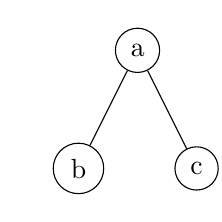
\begin{tikzpicture}

\node [circle,draw] (z){a}
  child {node [circle,draw] (a) {b}    
  }  
  child {node [circle,draw] (b) {c}
  };
\end{tikzpicture}
\caption{A 3 node binary tree.}

\end{center}
\end{figure}

Assume the probability of search for any of $a,b$, or $c$ is $\frac{1}{3}$. Under the three-way branch model, this can be done using exactly one comparison by asking if the key we are search for is less than $b$, equal to $b$, or strictly greater than $b$ and returning the correct key appropriately. Under a standard two-way branch model, this would require an extra comparison operation $\frac{2}{3}$ of the time as we can only distinguish one of the the three cases from the other two using a single two-way $<, >, \leq$ or $\geq$. This gives an expected cost of $1$ in the three-way branch model and $\frac{5}{3}$ in the two-way model. More specifically, each comparison can reveal $3$ bits of information in the three-way model, while only $2$ bits per comparison can be revealed in the two-way model. 

\section{Why Study Binary Search Trees}

Binary search trees are ubiquitous throughout computer science with numerous applications. The basic binary search tree has been built upon in many ways. AVL trees (named after creators AdelsonVelskii and Landis) were the first form of self-balancing binary search trees introduced \cite{adelsonvelskii1963algorithm}. The trees were invented by the pair in 1963 and maintain a height of $O(lg(n))$ where $n$ is the number of nodes in the tree during insertions and deletions (both of which take $O(lg(n))$ time). Improved self-balancing binary search trees followed in the form of red-black trees by Bayer in 1972 and splay trees by Sleator and Tarjan in 1985 \cite{bayer1972symmetric} \cite{sleator1985self}. Tango trees were invented in 2007 by Demaine et al. and provided the first $O(lg lg n)$ competitive binary tree \cite{demaine2007dynamic}. Here, $O(lg lg n)$ competitive means that the tango tree does at most $O(lg lg n)$ times more work (pointer movements and rotations) than an optimal offline tree. B trees are among the most commonly used binary tree variant and were invented in 1970 by Bayer and McCeight \cite{bayer1970organization}. \\

BST's and their extensions are integral to a large number of applications. For example, a BST variant known as the binary space partition is a method for recursviely subdividing space in order to store information in an easily accessible way. It is used extensively in 3D graphics \cite{schumacker1969study} \cite{paterson1992optimal}. Binary tries are similar to binary trees but only have values stored at the leaves. Binary tries are used routinely used in routers and IP lookup data structures \cite{song2010building}. Another example can be seen in the C++ std::map data structure, which is usually implemented using a red-black tree (another extension of binary search trees) in order to store its key-value pairs \cite{CppMap}. Finally, syntax trees (trees used in the parsing of various programming languages) are created using binary (and more complicated) tree structures. These trees are used in the parsing of written code during compilation \cite{louden1997compiler}.

\section{Overview}

In Chapter~\ref{Background and Related Work} I review previous work done in the areas of binary search trees, multiway trees, alphabetic trees and various models of external memory. In Chapter~\ref{An Improved Bound for the Modified Minimum Entropy Heuristic}, I re-examine the Modified Entropy Rule (ME) of G{\"u}ttler, Mehlhorn and Schneider \cite{guttler1980binary}. This is an $O(n^2)$ time, $O(n)$ space, algorithm for approximating the optimum binary search tree problem in the RAM model. The method works very well in practice, and the group had great experimental results, but unfortunately they could not bound the worst case expected cost as well as they would have hoped. While simpler solutions like the \textit{Min-max} and \textit{Weight Balanced} techniques of Bayer had worst case costs of at most $H+2$, the trio's ME technique had a worst case expected search cost of $c*H+2$ where $c \approx 1.08$ \cite{bayer1975improved} \cite{guttler1980binary}. I provide a new argument of the ME rule's worst case expected search cost and show that it is within a constant of entropy: at worst $H+4$. In Chapter~\ref{Approximate Binary Search in the Hierarchical Memory Model}, I move on to external memory models, examining the optimum binary search tree problem under the Hierarchical Memory Model of Aggarwal et al. \cite{aggarwal1987model} . I provide two $O(n*lg(m_1))$ time algorithms which have worst case expected cost of TODO FIX $C \leq (\lceil lg(m_1) \rceil * (\lfloor log_{m_1}(\frac{2}{min_{p,q}}) \rfloor + 1)) * W * (H + 1)$ WHERE TODO. The solution provided also gives a direct improvement over the solution Thite provided in the same work for HMM$_2$. In Chapter~\ref{Approximate Binary Search in the Hierarchical Memory with Block Transfer Model}, I extend my solutions to examine a more realistic model for external memory, the hierarchical memory with block transfers model (HMBTM). I use similar algorithms which run in TODO and give worst case expected search costs of TODO. In Chapter~\ref{BST over Multisets} I consider a variant of the optimum binary search tree problem (in the RAM model) where the set of probabilities given are from an unordered multiset. I show that a simple approach gives the optimum solution which is unique up to certain permutations. Finally, in Chapter~\ref{Conclusion and Open Problems}, I summarize my findings and discuss several problems which remain open.


\chapter{Background and Related Work} \label{Background and Related Work}



\section{Binary Search Trees}

After Knuth's initial examination of the optimum binary search tree problem in 1971 \cite{knuth1971optimum}, several others have examined the approximate version of the problem. Knuth's optimal solution requires $O(n^2)$ time and space which is too costly in many situations. While unable to bound an approximate algorithm within a constant of the optimal solution, many authors have been able to bound the cost based on the entropy of the distribution of probabilities, $H$. Specifically, 
\begin{center}
$H = \sum_{i=1}^{n} p_i*lg(\frac{1}{p_i}) + \sum_{j=0}^{n} q_i*lg(\frac{1}{q_j})$.
\end{center}
In 1975, Bayer showed that 
\begin{center}
$H-lg H-(lg e-1) \leq C_{Opt}$, $C_{Opt} \leq C_{WB} \leq H + 2$ and $C_{Opt} \leq C_{MM} \leq H + 2$
\end{center}
where $C_{Opt}, C_{WB}$, and $C_{MM}$ are costs for the optimal solution, as well as weight-balanced and min-max heuristic methods respectively \cite{bayer1975improved}. Weight-balanced and min-max costs heuristics are greedy and require both $O(n)$ time and $O(n)$ space to run. In 1980, G{\"u}ttler, Mehlhorn and Schneider presented a new heuristic, the Modified Entropy Rule (ME) \cite{guttler1980binary} which built upon the ideas of Horibe \cite{horibe1977improved}. G{\"u}ttler, Mehlhorn and Schneider gave empirical evidence that the heuristic out-performed others \cite{guttler1980binary}. While the heuristic took $O(n^2)$ time, it only required $O(n)$ space, a huge savings over the optimal solution. However, they were unable to prove that $C_{ME} \leq H+2$ (like previous weight-balanced and min-max heuristics) and settled with $C_{ME} \leq c_1*H+2$ where $c_1=\frac{1}{H(\frac{1}{3}, \frac{2}{3})} \approx 1.08$. I reexamine this method and provide a new bound of giving a new bound of $H+4$ in Chapter~\ref{An Improved Bound for the Modified Minimum Entropy Heuristic}. In 1993, De Prisco and De Santis presented a new heuristic for constructing a near-optimum binary search tree \cite{de1993binary}. The method is discussed in more detail in section~\ref{sec:deBST} and has an upper bounded cost of at most $H+1-q_0-q_n+q_{max}$ where $q_{max}$ is the maximum weight leaf node. This method was later updated by Bose and Dou\"{i}eb (and is also discussed in section~\ref{sec:deBST}) to have a worst case cost of 
\begin{center}
$H + 1 - q_0 - q_n + q_{max} - \sum_{i=0}^{m'} pq_{rank[i]}$
\end{center}
Here, $m'=max({2n-3P,P})-1 \geq \frac{n}{2} - 1$ where $P$ is the number of increasing or decreasing sequences in a left-to-right read of the access probabilities of the leaves and.  $pq_{rank[i]}$ is the $i^{th}$ smallest access probability among all keys and leaves except $q_0$ and $q_n$.

 
\section{Alphabetic Trees}

Optimum alphabetic trees is an important related problem worth discussing. Given a set of $n$ keys with various probabilities, we wish to build a binary search tree where every internal node has two children, leaves have no children, and the $n$ keys described are the leaves with minimum expected search cost. Here, the expected search cost is $\sum p_i * l_i*$ where $p_i$ is the probability of searching for leaf/key $i$ and $l_i$ is the leaf's level in the tree. The alphabetic ordering of the leaves must be maintained. This is the same as the binary search tree problem with all internal node weights zero.

In 1952, Huffman famously developed the Huffman tree, which solved the same problem without a left-to-right ordering constraint on leaves \cite{huffman1952method}. Gilbert and Moore examined the problem with the added alphabetic constraint and developed a $O(n^3)$ algorithm which solved the problem optimally \cite{gilbert1959variable}. Hu and Tucker gave a $O(n^2)$ time and space algorithm in 1971 \cite{hu1971optimal} which was improved by Knuth to take only $O(n lg n)$ time and $O(n)$ space in 1973 \cite{knuth1973sorting}. The original proof of Hu and Tucker was extremely complicated, but was later simplified by Hu \cite{hu1973new} and Hu et al. \cite{hu1979binary}. Garsia and Wachs gave an independent $O(n lg n)$ time, $O(n)$ space algorithm in 1977 \cite{garsia1977new}. This was shown to be equivalent to the Hu and Tucker algorithm in 1982 by Hu \cite{Hu1982Book} and also went through a proof simplification \cite{kingston1988new} by Kingston in 1988.

In 1991, Yeung proposed an approximate solution which solved the problem in $O(n)$ time and space \cite{yeung1991alphabetic}. The algorithm produced a tree with worst case cost $H + 2 - q_1-q_n$. This was later imporved by De Prisco and De Santis who created an $O(n)$ time algorithm which had a worst case cost of $H+1-q_0-q_n+q_{max}$ \cite{de1993binary}. The method was improved one more time by Bose and Dou\"{i}eb who improved upon Yeung's method by decreasing the bound by $\sum_{i=0}^m q_{rank[i]}$ where $m=max({n-3P,P})-1 \geq \frac{n}{4} - 1$, $P$ is the number of increasing or decreasing sequences in a left-to-right read of the access probabilities of the leaves and $q_{rank[i]}$ is the $i^{th}$ smallest access probability among all leaves except $q_0$ and $q_n$ \cite{bose2009efficient}. Replacing Yeung's method with the improved algorithm of Bose and Dou\"{i}eb in the De Prisco and De Santis algorithm gave the tightest bound seen so far of 
\begin{center}
$H+1+\sum_{i=1}^{n}q_i-q_0-q_n-\sum_{i=0}^m q_{rank[i]}$. 
\end{center}

\section{Multiway Trees} \label{sec:MWT}


Another related problem is the static k-ary or multiway search tree problem. It is similar to optimum binary search tree problem with the added constraint that up to $k$ keys can be placed into a single node, and cost of search within a node is constant. Multiway search trees maintain an ordering property similar to that of traditional binary search trees. Each key in every page in the subtree rooted at a specific location in a page $g$ (i.e. between two keys $k$ and $l$) must have its key lie between $k$ and $l$. Each internal node of the k-ary tree contains at least one and at most $k-1$ keys while a leaf node contains no keys. Successful searches end in an internal node while unsuccessful searches end in one of the $n+1$ leaves of the tree. The cost of search is the average path depth which is defined as:

\begin{center}
$\sum_{i=1}^{n} p_i(d_T(x_i)+1) + \sum_{j=0}^{n} q_j(d_T(x_{i-1},x_i))$
\end{center}

where $x_i$'s represent successful search keys, pairs $(x_{i-1},x_i)$ represent unsuccessful search "keys" and $d_T(x_i)$  or $d_T(x_{i-1},x_i)$ represent the depth of a specific successful or unsuccessful searches respectively.

Vishnavi et al. \cite{vaishnavi1980optimum}, and Gotlieb  \cite{gotlieb1981optimal} in 1980 and 1981 respectively independently solved the problem optimally in $O(k*n^3)$ time. In a slightly modified B-tree model (every leaf has same depth, every internal node is at least half full), Becker's 1994 work gave a $O(kn^{\alpha})$ time algorithm where $\alpha=2+log_k 2$ \cite{becker1994new}. Later, in 1997, Becker propsed an $O(Dkn)$ time algorithm where D is the height of the resulting tree\cite{becker1997construction}. The algorithm did not produce an optimal tree but was thought to be empirically close despite having no strong upper bound. In 2009, Bose and Dou\"{i}eb gave both an upper and lower bound on the optimal search tree in terms of the entropy of the probability distribution as well as an $O(n)$ time algorithm to build a near-optimal tree \cite{bose2009efficient}. Their bounds of:
\begin{center}
$\frac{H}{lg(2k-1)} \leq P_{OPT} \leq P_T \leq \frac{H}{lg k} + 1 + \sum_{i=0}^n q_i - q_0 - q_n - \sum_{i=0}^m q_{rank[i]}$
\end{center}
will be discussed in more detail in section~\ref{43} of this paper.

\section{Memory Models}

In the typical RAM model, we assume that all reads and writes from memory take a constant amount of time. While this is a valid assumption in many situations (both in the context of theory and programming) when dealing with very large data sets, this is simply not the case. A typical computer has a memory hierarchy with CPU registers, various levels of cache, RAM, SSD and/or hard drives. Each of these memory levels has increasing size but decreasing I/O speed. The difference between the levels is dramatic (reading from disk takes roughly a million times longer than accessing a CPU register) \cite{vitter2001external}. Moreover, many memory hierarchies allow blocks of memory to be moved quickly after a single word or cache line has been accessed. It is thus possible to take advantage of the locality of data during computations. It is thus imperative to consider memory I/O speeds, especially when the data set being worked on does not fit on internal memory. \textit{External memory} algorithms and data structures refer to those methods and structures which explicitly manage data placement and movement \cite{vitter2001external}. Various authors have created models to properly reflect the performance of such algorithms and data structrues, and I consider the optimum BST problem under two such models.

In Chapter~\ref{Approximate Binary Search in the Hierarchical Memory Model} I discuss the optimum binary search tree problem under the 1987 Hierarchical Memory Model of Aggarwal et al. \cite{aggarwal1987model}. The model is described thoroughly in section~\ref{The Hierarchical Memory Model}, but essentially provides an alternative to the classic RAM model. It simulates a memory hierarchy with various memory sizes and different access times for each type of memory. The model does have its shortcomings though as it does not provide us with the ability to move blocks of memory between these different memory types (as in a typical computer). 

In Chapter~\ref{Approximate Binary Search in the Hierarchical Memory with Block Transfer Model} I examine the same optimum binary search tree problem but under the extended Hierarchical Memory with Block Transfer Model of Aggarwal, Chandra, and Snir \cite{aggarwal1987hierarchical}. This model extends the previous model, proving a slightly less artificial setting by allowing for contiguous blocks of memory to be copied from one location to another for a cheaper price. The cost of this copy equal to the cost to access the most expensive location being copied, (to or from) plus the size of the block. \\

As explained in the survey of Vitter, several other models of external memory have followed \cite{vitter2001external}. Work has been done to consider models with parallelism. Vitter and Shriver built upon the HMM and HMBTM models of Aggarwal et al. \cite{aggarwal1987model}, \cite{aggarwal1987hierarchical} in order to allow parallelism \cite{vitter1994algorithms}. The model connects $P$ parallel memory hierarchies at their base memory level. In 1994, Alpern et al. introduced the uniform memory hierarchy \cite{alpern1994uniform}. The model considers considers block size and bandwidth between memory levels, and allows for simultaneous transfer between pairs of memory levels. This model was considered with additional parallelization by Vitter and Nodine \cite{vitter1993large}.


Cache-oblivious algorithms were introduced by Frigo, Leiserson, Prokop and Ramachandran in 1999 \cite{frigo1999cache}. The model used is the ideal-cache model which has a two-level memory hierarchy. The internal memory (cache) has $Z$ words and the main memory is arbitrarily large. The cache is divided into cache lines of size $L$ and it is assumed that $Z=\Omega(L^2)$. Frigo et. al examined the fast fourier transform and matrix multiplication under this model. Many others have since used this model and examined problems in a cache-oblivious setting such as the cache-oblivious b-trees of bender et. al \cite{bender2000cache}, the funnel heap of Brodai et. al \cite{brodai2002funnel}, or the locality preserinv cache-oblivious dynamic dictionary of Bender et. al \cite{bender2002locality}.

A complete and thorough explanation of memory hierarchies (especially those considered before cache oblivious settings) can be found in the survey of Vitter \cite{vitter2001external}.



\chapter{An Improved Bound for the Modified Minimum Entropy Heuristic}\label{An Improved Bound for the Modified Minimum Entropy Heuristic}

\section{Preliminaries}

Recall that $H = \sum_{i=1}^{n} p_i*lg(\frac{1}{p_i}) + \sum_{j=0}^{n} q_i*lg(\frac{1}{q_j})$. We also use $H(x_1,x_2,...,x_n)$ to describe the entropy of probability distribution $(x_1, x_2, ...., x_n)$. For sub tree $t$, we let $p_t$ be its total probability. $P_{L}(p_i)$ and $P_{R}(p_i)$ are probabilities of searching for a word lexicographically before or after (respectively) word $B_i$. $P_{L_t}(p_i)=\frac{P_L(p_i)}{p_t}$ and $P_{R_t}(p_i)=\frac{P_R(p_i)}{p_t}$ are these same probabilities normalized for sub tree $t$. Similarly, $P_{L_t}(q_j)$ and $P_{R_t}(q_j)$ describe the normalized probabilities of searching for a word before or after (respectively) the lexicographic gap between words $B_j$ and $B_{j+1}$. We let $E_t=H(P_{L_t}(p_i), \frac{p_i}{p_t}, P_{R_t}(p_i))$ be the local entropy of a sub tree $t$ rooted at word $B_i$.  

\section{The Modified Entropy Rule}

As described in \cite{guttler1980binary}, the heuristic greedily chooses the word $B_i$ as the root such that $H(P_{L_t}(p_i), \frac{p_i}{p_t}, P_{R_t}(p_i))$ is maximized. There are two exceptions to this rule. First, if there exists $p_i$ such that $\frac{p_i}{p_t} > max(P_{L_t}(p_i), P_{R_t}(p_i))$ we always select $B_i$ as the root. Moreover, if there exists $q_j$ such that $\frac{q_j}{p_t} > max(P_{L_t}(q_j), P_{R_t}(q_j))$ then we select the root from among $B_j$ and $B_{j+1}$. $B_j$ is chosen if $P_{L_t}(q_j) > P_{R_t}(q_j)$ and $B_{j+1}$ is chosen otherwise. Since it takes linear time and constant space to find the all of the optimal local entropy splits in each level of the tree, the algorithm takes $O(n^2)$ time and $O(n)$ space.  \\

\section{ME is within 4 of Entropy}

\begin{lem}
When using the ME Rule to choose the root $B_r$ of a binary search tree $t$ with total probability $p_t$, one of the following three cases must occur: \\
1) $E_t \geq 1-2 \frac{p_r}{p_t}$ \\
2) There exists $q_i$ such that $\frac{q_i}{p_t} > max(P_{L_t}(q_i), P_{R_t}(q_i))$\\
3)  $max(P_{L_t}(p_r), P_{R_t}(p_r)) < \frac{4}{5} p_t$\\
\end{lem}
\begin{proof}
Suppose there exists some $p_i$ such that $\frac{p_i}{p_t} > max(P_{L_t}(p_i), P_{R_t}(p_i))$. By the ME Rule, it must be selected as the root and thus $p_r=p_i$. Moreover, both $P_{L_t}(p_i)$ and $P_{R_t}(p_i))$ must be less than one half. As shown in \cite{gallager1968information} $H(x,1-x) \geq 2x$ when $x<\frac{1}{2}$. Thus we have: \\
$E_t \geq H( max(P_{L_t}(p_i), P_{R_t}(p_i)), 1-max(P_{L_t}(p_i), P_{R_t}(p_i))$ \\
$ \geq 2*max(P_{L_t}(p_i), P_{R_t}(p_i))$ \\ $ \geq 1-\frac{p_i}{p_t}$ \\ 
$ \geq 1-2 \frac{p_i}{p_t} \geq 1-2 \frac{p_r}{p_t}$ \\
 as required. \\
 
 If we do not have some $p_i$ such that $\frac{p_i}{p_t} > max(P_{L_t}(p_i), P_{R_t}(p_i))$ but do have some $p_i$ such that $P_{L_t}(p_i) \leq \frac{1}{2}p_t$ and $P_{R_t}(p_i) \leq \frac{1}{2}p_t$) then we have: \\
 $E_t \geq H(P_{L_t}(p_i), \frac{p_i}{p_t} , P_{R_t}(p_i)$ where $0 \leq P_{L_t}(p_i) \leq 0.5$, $0 \leq \frac{p_i}{p_t} \leq 0.5$ and $0 \leq P_{R_t}(p_i) \leq 0.5$  and we know that \\
 $H(P_{L_t}(p_i), \frac{p_i}{p_t} , P_{R_t}(p_i)) \geq H(1/2, 1/2) = 1$ in this case.
 Thus, $E_t \geq 1-2p_r$ as required. \\
 
 Otherwise, we must have some $q_i$ spanning the middle of the data set (i.e. $P_{L_t}(q_i) < \frac{1}{2}p_t$ and $P_{R_t}(q_i) < \frac{1}{2}p_t$). Suppose that case 2) does not occur: there does not exist a $q_i$ such that $\frac{q_i}{p_t} > max(P_{L_t}(q_i), P_{R_t}(q_i))$. Then, we have that \\ $max(P_{L_t}(p_i), P_{R_t}(p_i)) \geq min(P_{L_t}(p_i), P_{R_t}(p_i))$ and \\ $max(P_{L_t}(p_i), P_{R_t}(p_i)) \geq q_i$ \\ Thus, $max(P_{L_t}(p_i), P_{R_t}(p_i)) \geq 1/3$ and by our assumption $max(P_{L_t}(p_i), P_{R_t}(p_i)) < \frac{1}{2}$. \\
 So, as in the proof of table 3 (5.3) in \cite{guttler1980binary}\\
 $E_t \geq H(1/3, 2/3) \approx 0.92$. \\

Now also suppose that case 1) does not occur. 
$\implies E_t < 1-2\frac{p_r}{q_t}$ \\
$\implies \frac{p_r}{q_t} < \frac{1-H(\frac{1}{3}, \frac{2}{3})}{2} \approx 0.04$ \\
Suppose that $max(P_{L_t}(p_r), P_{R_t}(p_r)) \geq \frac{4}{5} p_t$ then we have \\
$E_t \leq H(\frac{4}{5}, \frac{1-H(\frac{1}{3}, \frac{2}{3})}{2}, \frac{1}{5}-\frac{1-H(\frac{1}{3}, \frac{2}{3})}{2}) \approx 0.87 < H(\frac{1}{3}, \frac{2}{3}) \leq E_t$ \\ 
a contradiction. \\
Thus, if we do not have case 1) or 2), we must have case 3). Since this is our last remaining case, this completes the proof.
 

\end{proof}

Before we examine the main theorem I show a small claim.

\newtheorem{claim}{Claim}
\begin{claim}
$H(\frac{1}{2}-\frac{1}{2} x, \frac{1}{2} + \frac{1}{2} x) \geq 1- \frac{4}{5} (x)^2$ when $0 < x < \frac{1}{2}$
\end{claim}

\begin{proof}
In order to prove the claim, we find the minimum of \\
$H(\frac{1}{2}-\frac{1}{2} x, \frac{1}{2} + \frac{1}{2} x) - (1 - \frac{4}{5} (x)^2)$ when $0 < x < \frac{1}{2}$. \\
To do this we take the derivative with respect to $x$. \\
Let $F= H(\frac{1}{2}-\frac{1}{2} x, \frac{1}{2} + \frac{1}{2} x) - (1 - \frac{4}{5} (x)^2)$ \\
$\implies F = - (\frac{1}{2}-\frac{1}{2} x)* lg(\frac{1}{2}-\frac{1}{2} x) - (\frac{1}{2} + \frac{1}{2} x)*lg(\frac{1}{2} + \frac{1}{2} x) - (1 - \frac{4}{5} (x)^2)$ \\
$\implies F' = lg(\frac{1}{2}-\frac{1}{2} x) - lg(\frac{1}{2} + \frac{1}{2} x) + \frac{8}{5}x$ \\ 
The only root here occurs when $x = 0$. Thus, we check when $x \rightarrow 0$ and $x \rightarrow \frac{1}{2}$. We note that: \\
$F' \rightarrow 0^{+}$ when $x \rightarrow 0$ and \\
$F' \rightarrow \approx 0.0112781 > 0$ when $x \rightarrow \frac{1}{2}$. \\
Thus, $H(\frac{1}{2}-\frac{1}{2} x, \frac{1}{2} + \frac{1}{2} x) - (1 - \frac{4}{5} (x)^2) > 0$ for $ 0 < x < \frac{1}{2}$ which proves the claim.
\end{proof} 


\begin{thm}
$C_{ME} \leq H + 4$
\end{thm}

\begin{proof}
This uses a similar style to the proof of theorem 4.4 in \cite{bayer1975improved}.
We will bind each $E_t$ for each sub tree of our BST on a case by case basis using the cases of \textbf{Lemma 3.3.1}.\\
If case 1 occurs, we obviously have that \\
$E_t \geq 1-2 \frac{p_r}{p_t}$ \\
Note that this can only happen once for each word (a word can only be root once). \\

While it wasn't explicitly stated, in \textbf{Lemma 3.3.1} it was shown that if some $p_i$ spans in the middle of the data set, $P_{L_t}(p_i) \leq \frac{1}{2}p_t$ and $P_{R_t}(p_i) \leq \frac{1}{2}p_t$, then regardless of whether or not $\frac{p_i}{p_t} > max(P_{L_t}(p_i), P_{R_t}(p_i))$, we can still show that case 1 occurs. Suppose for the remainder of the proof that there is no such middle-spanning $p_i$.

Let $q_m$ be the unique middle gap (i.e. $P_{L_t}(q_m) < \frac{1}{2} p_t$ and $P_{R_t}(q_m) < \frac{1}{2} p_t$) when case 2 or 3 occurs. When case 2 occurs we have that: \\
$E_t \geq H(\frac{1}{2}-\frac{1}{2} \frac{q_m}{p_t}, \frac{1}{2} + \frac{1}{2} \frac{q_m}{p_t}) \geq 2(\frac{1}{2}-\frac{1}{2} \frac{q_m}{p_t})=1-\frac{q_m}{p_t}$. \\
Note that by the definition of the ME Rule, when this occurs, $q_m$ must be a leaf of depth at most 2. Thus, this condition can only happen twice for each $q_m$. \\

When case 2 does not occur (and we have a $q_m$ spanning the middle) we must have case 3. This gives us: \\
$E_t \geq H(\frac{1}{2}-\frac{1}{2} \frac{q_m}{p_t}, \frac{1}{2} + \frac{1}{2} \frac{q_m}{p_t})$ \\
By subbing in $\frac{q_m}{p_t}$ for $x$ we know from \textbf{Claim 1} that:
$\implies E_t \geq 1- \frac{4}{5} (\frac{q_m}{p_t})^2$\\

As in \cite{bayer1975improved} we define a $b_t$ for each sub tree $t$ as follows: \\
let $b_t=2p_r$ for case 1. \\
let $b_t=2q_m$ for case 2. \\
let $b_t=\frac{q_m^2}{p_t}$ for case 3. \\
Note that, in 1975 Bayer showed that: \\
$C = \sum_{t \in S_T} p_t$ and $H = \sum_{t \in S_T} P_t E_t $ Where $S_T$ is the set of all sub trees of our tree (\textbf{Lemma 2.3} \cite{bayer1975improved}).
Thus, we have\\
$H = \sum_{t \in S_T} P_t E_t \geq \sum_{t \in S_T} P_t - \sum b_t = C - \sum b_t$ \\
$ \implies C \leq H + \sum b_t$ \\

As mentioned above, cases 1 and 2 can only occur once and twice respectively. Case 3 however, can occur many times, but each time it occurs, $\frac{q_m}{p_t}$ must decrease by a factor of $\frac{5}{4}$ since $max(P_{L_t}(p_r), P_{R_t}(p_r)) < \frac{4}{5} p_t$ (we recursively examine a smaller sub tree). Moreover, if $\frac{q_m}{p_t} > \frac{1}{2}$ then we will have case 2. Let $S_m$ be the set of all sub trees $t$ for which $q_m$ is the middle gap and case 3 only applies. We have that \\
$C \leq H + \sum b_t = H + 2 \sum\limits_{r = 1}^n p_r + 2 \sum\limits_{m = 0}^n q_m + \sum\limits_{m = 0}^n \sum\limits_{t \in S_m} \frac{4}{5}\frac{q_m^2}{p_t}$ \\ 
By factoring out $q_m$ and examining only cases up to $\frac{q_m}{p_t} = \frac{1}{2}$ we get: \\
$\implies C \leq H + 2 + \sum\limits_{m = 0}^n \frac{4}{5} q_m \sum\limits_{x=0}^{\infty} \frac{1}{2} * (\frac{4}{5}) ^ x$ \\
$\implies C \leq H + 2 + \sum\limits_{m = 0}^n \frac{4}{5}q_m (\frac{1}{2} * \frac{1}{1-\frac{4}{5}})$ (geometric series) \\
$\implies C \leq H + 4$ \\

\end{proof}

\chapter{Approximate Binary Search in the Hierarchical Memory Model}\label{Approximate Binary Search in the Hierarchical Memory Model}
 
\section{The Hierarchical Memory Model}\label{The Hierarchical Memory Model}

The Hierarchical Memory Model (HMM) was proposed in 1987 by Aggarwal et al. as an alternative to the classic RAM model \cite{aggarwal1987model}. It was intended to better model the multiple levels of the memory hierarchy. The model has an unlimited number of registers, $R_1, R_2, ...$ each with its own location in memory (a positive integer). In the first version of the model, accessing a register at memory location $x_i$ takes $\lceil lg(x_i) \rceil$ time. Thus, computing $f(a_1, a_2, ..., a_n)$ takes time $\sum_{i=1}^{n} \lceil lg(location(a_i)) \rceil$. The original paper also considered arbitrary cost functions $f(x)$. We will use the cost function as was explained in Thite's thesis \cite{thite2008optimum}. Here, $\mu (a)$ is the cost of accessing memory location $a$. We have a series of memory sizes $m_1, m_2, ..., m_l$. Each memory level has a finite size except $m_l$ which we assume has infinite size. Each memory level has an associated cost of access $c_1, c_2, ..., c_l$. We assume that $c_1 < c_2 < ... < c_l$. 

\begin{center}$\mu (a) = c_i if \sum_{j = 1}^{i-1}m_j  < a \leq \sum_{j = 1}^{i}m_j$. \end{center}

Thite notes that typical memory hierarchies have decreasing sizes for faster memory levels (moving \textit{up} the memory hierarchy). We make the same assumption:
\begin{center}
$m_1 < m_2 < ... < m_l$
\end{center}
Unlike Thite, we also explicitly assume that successive memory level sizes divide one another evenly:
\begin{center}
$\forall i \in  \{1,2,...,l-1\}$, $m_i \mid m_{i+1}$.
\end{center}

\section{Thite's Optimum Binary Search Trees on the HMM Model}

Thite's thesis provided solutions to several problems in the HMM and the related HMM$_2$ models \cite{thite2008optimum}. He first provided an optimal solution to the following problem (known as \textbf{Problem 5} in the work):\\


\textbf{Problem [Optimum BST Under HMM].} Suppose we are given a set of $n$ ordered keys $x_1, x_2, ..., x_2$ with associated probabilities of search $p_1, p_2, ..., p_n$, as well as $n+1$ ranges $(- \infty, x_1), (x_1, x_2), ..., (x_{n-1}, x_n), (x_n, \infty)$ with associated probabilities of search $q_0, q_1, ..., q_n$. The problem is to construct a binary search tree $T$ over the set of keys and compute a memory assignment function $\phi : V (T) \rightarrow {1, 2, ..., n}$ that assigns nodes of $T$ to memory locations such that the expected cost of a search is minimized under the HMM model \cite{thite2008optimum}.\\


He provided three separate optimum solutions; \textbf{Parts}, \textbf{Trunks}, and \textbf{Split}. These algorithms have various use cases and running of times $O(\frac{2^{h-1}}{(h-1)!}* n^{2h+1})$, $O(\frac{2^{n-m_h}*(n-m_h+h)^{n-m_h}*n^3}{(h-2)!})$ and $O(2^n)$ respectively. Here, $h$ is the minimum memory level such that all $n$ keys can fit on memories $\leq h$: \\
\begin{center}
$min(h \in \{1,..,l\} ): n \leq \sum_{i = 1}^{h}m_i$
\end{center}


 In the following sections, I will provide two approximate solutions to this problem that run in time $O(n*lg(m_1))$ and provide an upper bound on their expected search costs.  \\

Thite also considered the same problem under the related HMM$_2$ model. This model assumes there are simply two levels of memory of size $m_1$ and $m_2$ with costs of access $c_1$ and $c_2$ where $c_1 < c_2$. Thite provided an optimal solution to this problem (named \textbf{TwoLevel}) which ran in time $O(n^5)$. It ran in $o(n^5)$, if $m_1 \in o(n)$, and in $O(n^4)$ if $m_1 \in O(1)$. He also gave an $O(nlg n)$ time approximate solution with an upper bounded expected search cost of $c_2(H+1)$. The solution I provide under the HMM model also provides an improvement over Thite's approximate algorithm in both running time and expected cost under the HMM$_2$ model.


\section{Efficient Near-Optimal Multiway Trees of Bose and Dou\"{i}eb}\label{43}

In order to approximately solve the optimum BST problem under the HMM model, I will use a multiway search tree construction algorithm of Bose and Dou\"{i}eb. In 2009, the duo devised a new method with linear running time (independent of the size of a node in tree) and with the best expected cost to date \cite{bose2009efficient}. The group was able to prove that:
\begin{center}
$\frac{H}{lg(2k-1)} \leq P_{OPT} \leq P_T \leq \frac{H}{lg k} + 1 + \sum_{i=0}^n q_i - q_0 - q_n - \sum_{i=0}^m q_{rank[i]}$
\end{center}
Here, H is the entropy of the probability distribution, $P_{OPT}$ is the average path-length in the optimal tree, $P_T$ is the average path length of the tree built using their algorithm and $m=max({n-3P,P})-1 \geq \frac{n}{4} - 1$. $P$ is the number of increasing or decreasing sequences in a left-to-right read of the access probabilities of the leaves. Moreover, $q_{rank[i]}$ is the $i^{th}$ smallest access probability among all leaves except $q_0$ and $q_n$. Finally, $k$ is the size of a node in the tree. \\

As described in the section~\ref{sec:MWT}, in the multiway search tree problem we are given $n$ ordered keys with weights $p_0, ..., p_n$ as well as $n+1$ weights of unsuccessful searches $q_0,...,q_n$. We often refer to "keys" representing the gaps as $(x_{i-1},x_i)$ to be mean the "key" associated with a search between key $x_{i-1}$ and $x_i$. We attempt to build a minimum cost tree where $k$ keys fit inside a single node.\\
 
 The algorithm occurs in three steps. First, a new distribution is created by distributing all leaf weights to appropriate internal nodes. Without going into great detail, essentially an examination of the peaks and valleys of the probability distribution of the leaf weights is used to do this weight reassignment. After this, the new probability distribution is made into a k-ary tree using a greedy recursive algorithm. The algorithm recursively chooses the $l \leq k$ elements to go in the root node such that each child's subtree will have probability of access of at most $1/k$. After this internal key tree has been completed, leaf nodes are reattached. Their algorithm's design allows them to bound the depth of keys and leaves. This ultimately allows them to achieve the bounds they have described. 

\section{Algorithm ApproxMWPaging}\label{Algorithm ApproxMWPaging}

First, we need a lemma about converting a multiway search tree to a binary search tree. For the sake of clarity, we will call what are typically known as \textit{nodes} of the multiway tree \textit{pages}. This represents how various items of our search tree will fit onto pages of our memory hierarchy. We maintain the notion of calling individual items \textit{keys}.

\begin{lem}\label{MWTBSTLem}
Given a multiway tree $T'$ with page size $k$ and $n$ keys, where keys are associated with a probability distribution of successful and unsuccessful searches as in Knuth's original optimum binary search tree problem, we can create a BST $T$ where each key in a given page $g \in T'$ forms a connected component in $T$ in $O(nlg(k))$ time.
\end{lem}

\begin{proof}
For each page $g$, we sort its keys by value and create a complete BST $B$ over the keys. We create an ordering over all potential locations where keys could be added to the tree from left to right. All keys in all descendant pages of a page $g$ in a specific subtree rooted at a child of $g$ will lie in a specific range. There are at most $k+1$ of these ranges (since our page has at most $k$ keys). These ranges will precisely correspond to the at most $k+1$ locations where a new child key could be added to $B$. We note that we cannot add new children to keys which correspond to unsuccessful searches. We order these locations from left to right and attach root keys from the newly created BST's of each of the ordered (left to right) children of $g$. These will all be valid connections since each child of $g$ has keys in these correct ranges, and combining BST's in this fashion produces a valid BST. We perform a sort of $O(k)$ items (in time $O(klg(k))$) $O(n/k)$ times, and make $O(n)$ new parent child connections, giving us total time $O(n lg(k)$.
\end{proof}

In order to approximately solve the optimum BST problem under the HMM model, we will do the following: \\

1) First, we create a Multiway Tree $T'$ using the algorithm of Bose and Dou\"{i}eb. This takes $O(n)$ time with our node size equal to $m_1$ (the smallest level of our memory hierarchy) \cite{bose2009efficient}. \\

2) Inside each page (node of the multiway tree $T'$), we create a balanced binary search tree (ignoring weights). We use a simple greedy approach where we sort the keys, then recursively select the middle key as the root.  We call each of these $T'_k$ for $k \in {1,...,\lceil n/m_1 \rceil}$. This takes $O(m_1*lg(m_1))$ time per page, of which there are at most $O(n/m_1)$ giving us $O(n*lg(m_1))$ time total. \\

3) In order to make this into a proper binary search tree, we must connect the $O(n/m_1)$ BST's we have made as described in Lemma~\ref{MWTBSTLem}. From $T'$, we create a BST $T$. This takes $O(n*lg(m_1))$ time. \\

4) We pack keys into memory in a breadth first search order of $T$ starting from the root. This takes $O(n)$ time. \\

We are left with a binary search tree which has been properly packed into our memory in total time $O(n*lg(m_1))$.

\pagebreak
\begin{figure}[H]

% Set the overall layout of the tree
\tikzstyle{level 1}=[level distance=3cm, sibling distance=3cm]
\tikzstyle{level 2}=[level distance=3cm, sibling distance=3cm]

\begin{center}
\begin{subfigure}[b]{0.36\textwidth}

\scriptsize


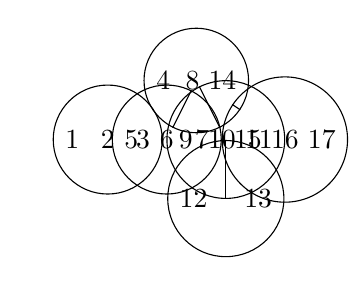
\begin{tikzpicture}[scale=0.5]

\node [circle,draw] (z){4\: 8 14}
  child {node [circle,draw] (a) {1\: \:2\: \:3}    
  }  
  child {node [circle,draw] (b) {5\: \:6\: \:7}
  }  
  child {node [circle,draw] (c) {9\: 10 11}
    child {node [circle,draw] (e) {12 \:\:\: 13}}
  }
  child {node [circle,draw] (d) {15 16 17}
  };

\end{tikzpicture}
\caption{Phase 1)}
\end{subfigure}
\end{center}

\vspace{3em}

% Set the overall layout of the tree
\tikzstyle{level 1}=[level distance=3cm, sibling distance=3.5cm]
\tikzstyle{level 2}=[level distance=3cm, sibling distance=3.5cm]

\tikzset{smnode/.style={level 1/.style={level distance=1cm, sibling distance=1cm}, circle, draw}}
\tikzstyle{level 1}=[level distance=3cm, sibling distance=3.5cm]
\tikzstyle{level 2}=[level distance=3cm, sibling distance=3.5cm]
\tikzstyle{level 3}=[level distance=1cm, sibling distance=1cm]
\begin{center}
\begin{subfigure}[b]{0.82\textwidth}
\begin{tikzpicture}
\scriptsize
\node[circle,draw] (z){
	\tikzstyle{level 1}=[level distance=1cm, sibling distance=1cm]
	\begin{tikzpicture}
	\node [draw,circle] (zZ){8}
  	child {node [draw,circle] (Za) {4}    
  	}  
  	child {node [draw,circle] (Zb) {14}
  	};
	\end{tikzpicture}
}	
	  	
  child {node [circle,draw] (a) {
	\tikzstyle{level 2}=[level distance=1cm, sibling distance=1cm]
	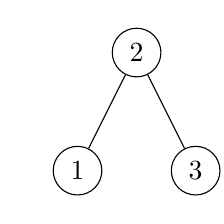
\begin{tikzpicture}
	\node [circle,draw] (z){2}
  	child {node [circle,draw] (a) {1}    
  	}  
  	child {node [circle,draw] (b) {3}
  	};
	\end{tikzpicture}  
  }edge from parent[shorten <=1.02cm] 
  }  
  child {node [circle,draw] (b) {
	\tikzstyle{level 2}=[level distance=1cm, sibling distance=1cm]
	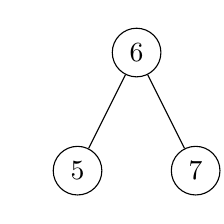
\begin{tikzpicture}
	\node [circle,draw] (z){6}
  	child {node [circle,draw] (a) {5}    
  	}  
  	child {node [circle,draw] (b) {7}
  	};
	\end{tikzpicture}   
  }edge from parent[shorten <=1.02cm]
  } 
  child {node [circle,draw] (c) {
	\tikzstyle{level 2}=[level distance=1cm, sibling distance=1cm]
	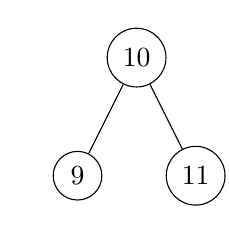
\begin{tikzpicture}
	\node [circle,draw] (z){10}
  	child {node [circle,draw] (a) {9}    
  	}  
  	child {node [circle,draw] (b) {11}
  	};
	\end{tikzpicture}  
  	}
  	child {node [circle,draw] (asdf) {
  	\tikzstyle{level 2}=[level distance=1cm, sibling distance=1cm]
	\begin{tikzpicture} 
	  	\node [smnode] (zz){12}
	  	child {node [circle,draw=none] {}edge from parent[draw=none]}	  	
  		child {node [smnode] (asaa) {13}    
  		}; 		
	\end{tikzpicture}	
  	}
  	}  	    
  edge from parent[shorten <=0.97cm]
  }
  child {node [circle,draw] (d) {
	\tikzstyle{level 2}=[level distance=1cm, sibling distance=1cm]
	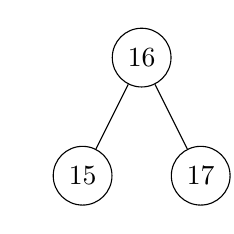
\begin{tikzpicture}
	\node [circle,draw] (z){16}
  	child {node [circle,draw] (a) {15}    
  	}  
  	child {node [circle,draw] (b) {17}
  	};
	\end{tikzpicture}   
  }edge from parent[shorten <=0.97cm]
  };
\end{tikzpicture}
\caption{Phase 2)}
\end{subfigure}
\end{center}

\end{figure}

\clearpage

\begin{figure}[H]
\begin{center}
\scriptsize

\tikzstyle{level 1}=[level distance=1cm]
\tikzstyle{level 2}=[level distance=1cm]
\tikzstyle{level 3}=[level distance=1cm]
\begin{subfigure}[b]{0.72\textwidth}

\begin{tikzpicture}[level/.style={sibling distance=60mm/#1}]
\node [circle,draw] (z){8}
  child {node [circle,draw] (a) {4}    
	child {node [circle,draw] (b) {2}
		child {node [circle,draw] (c) {1}}
		child {node [circle,draw] (d) {3}}}  
  	child {node [circle,draw] (e) {6}
		child {node [circle,draw] (f) {5}}
		child {node [circle,draw] (g) {7}}}  
  }  
  child {node [circle,draw] (h) {14}    
	child {node [circle,draw] (i) {10}
		child {node [circle,draw] (j) {9}}
		child {node [circle,draw] (k) {11}
			child {node [circle,draw=none] (o) {}edge from parent[draw=none]}
			child {node [circle,draw] (o) {12}
				child {node [circle,draw=none] (s) {}edge from parent[draw=none]}				
				child {node [circle,draw] (p) {13}
		}}}}  
  	child {node [circle,draw] (l) {16}
		child {node [circle,draw] (m) {15}}
		child {node [circle,draw] (n) {17}}}  
  };

\end{tikzpicture}
\caption{Phase 3)}



\end{subfigure}
\end{center}


\begin{center}
\scriptsize

\begin{subfigure}[b]{0.72\textwidth}


\begin{center}
    \begin{tabular}{ | l | l | l | p{5cm} |}
    \hline
    Memory Location & Node & Left Child Location & Right Child Location \\ \hline
    1  & 8  & 2    & 3    \\ \hline
    2  & 4  & 4    & 5    \\ \hline
    3  & 14 & 6    & 7    \\ \hline
    4  & 2  & 8    & 9    \\ \hline
    5  & 6  & 10   & 11   \\ \hline
    6  & 10 & 12   & 13   \\ \hline
    7  & 16 & 14   & 15   \\ \hline
    8  & 1  & NULL & NULL \\ \hline
    9  & 3  & NULL & NULL \\ \hline
    10 & 5  & NULL & NULL \\ \hline
    11 & 7  & NULL & NULL \\ \hline
    12 & 9  & NULL & NULL \\ \hline
    13 & 11 & NULL & 16   \\ \hline
    14 & 15 & NULL & NULL \\ \hline
    15 & 17 & NULL & NULL \\ \hline
    16 & 12 & NULL & 17   \\ \hline
    17 & 13 & NULL & NULL \\ \hline
    \end{tabular}
\end{center}

\caption{Phase 4)}
\end{subfigure}
\end{center}


\caption{An example of the first three steps of the ApproxMWPaging Algorithm.}
\end{figure}


\section{Expected Cost ApproxMWPaging} \label{45}

First, we bound the depth of nodes in our BST $T$. The depth of a key $x_i$ (denoted $(x_{i-1}, x_i)$ for unsuccessful searches) is defined as $d_T(x_i)$ ($d_T(x_{i-1},x_i)$). Note that depth is the number of edges between a node and the root (i.e. the depth of the root is $0$). As in the work of Bose and Dou\"{i}eb, let $m=max({n-3P,P})-1 \geq \frac{n}{4} - 1$ where $P$ is the number of increasing or decreasing sequences in a left-to-right read of the access probabilities of the leaves \cite{bose2009efficient}.

\begin{lem} \label{451}
For a key $x_i$,
\begin{center} $d_T(x_i) \leq lg(\frac{1}{p_i})$. \end{center}
For a key $(x_{i-1},x_i)$,
\begin{center} $d_T(x_{i_1},x_i) \leq lg(\frac{1}{q_i}) + 2$ for all leaves, and\\
 $d_T(x_{i_1},x_i) \leq lg(\frac{1}{q_i}) + 1$ for at least $m$ of them (and the two extremal leaves). \end{center}
  
\begin{center}

\end{center}

\end{lem}

\begin{proof}
First we note that in the tree $T'$ we build using Bose and Dou\"{i}eb's multiway tree algorithm, the maximum depth of keys (call this $d_{T'}(x_i), d_{T'}(x_{i-1},x_i)$) for a page size $m_1$ is \cite{bose2009efficient}:
\begin{center} $d_{T'}(x_i) \leq \lfloor log_{m_1}(\frac{1}{p_i}) \rfloor$. \end{center} 
\begin{center} $d_{T'}(x_{i_1},x_i) \leq \lfloor log_{m_1}(\frac{2}{q_i}) \rfloor + 1$ for all leaves, and\\
 $d_T(x_{i_1},x_i) \leq \lfloor log_{m_1}(\frac{1}{q_i}) \rfloor + 1$ for at least $m$ of them (and the two extremal leaves). \end{center}
As explained in the paper, these follow from Lemmas 1 and 2 of Bose and Dou\"{i}eb \cite{bose2009efficient}.

Inside a page, we make a balanced (ignoring weight) BST, so each key has a depth within a page of at most $\lfloor lg(m_1) \rfloor$. Since our algorithm always connects the root of the BST made for page to a key in the BST made for the page's parent, a key $x_i$ has a \textit{page depth} (the number of unique pages accessed in order to access the key) of at most  the bounds on $d_{T'}(x_i)$ and $d_{T'}(x_{i_1},x_i)$ described. Since we will examine at most $\lceil lg(m_1) \rceil$ keys within any one page (and only 1 key in a leaf page) a key's depth is at most \\
$d_T(x_i) \leq \lfloor lg(m1) \rfloor \lfloor log_{m_1}(\frac{1}{p_i}) \rfloor$ \\
$\implies d_T(x_i) \leq lg(m1)*log_{m_1}(\frac{1}{p_i})$ \\
$\implies d_T(x_i) \leq lg(\frac{1}{p_i})$. \\
For an unsuccessful search \\
$d_T(x_{i_1},x_i) \leq \lfloor lg(m1) \rfloor \lfloor log_{m_1}(\frac{2}{q_i}) \rfloor + 1$ \\
$\implies d_T(x_{i_1},x_i) \leq lg(m1)*log_{m_1}(\frac{2}{q_i}) + 1$ \\
$\implies d_T(x_{i_1},x_i) \leq lg(\frac{1}{q_i}) + 2$ for all leaves, and \\
$\implies d_T(x_{i_1},x_i) \leq lg(\frac{1}{q_i}) + 1$ for at least $m$ of them (and the two extremal leaves).


\end{proof}

We now describe the cost of searching for a key located at deepest part of tree $T$: $W$. Let $m'_j = \sum_{k \leq j} m_j$. We define $m'_0 = 0$. As defined previously we let $l$ be the smallest $j$ such that $m'_j > n$. Let $H(T)$ be the height of $T$.


\begin{lem} \label{452} \hspace{1cm} \\
$W \leq \sum_{i=1}^{l-1} (\lfloor lg(m'_i+1) \rfloor - \lfloor lg(m'_{i-1}+1) \rfloor)*c_i+ (H(T) - \lfloor lg(m'_{l-1}+1) \rfloor)*c_l$
\end{lem}


\begin{proof}
Consider the accessing each key along the path from the root to the deepest key in $T$. We will examine $H(T)$ keys. We will access one key at depth $0$, one key at depth $1$, and so on. Because the tree is packed into memory in BFS order, a key a depth $i$ will be at memory location at most $2^i-1$. Now, consider how many levels of the binary search tree $T$ will fit in $m_1$. In order for all keys of depth $i$ (and higher) to be in $m_1$ we need:
\begin{center}
$2^i-1 \leq m_1 \implies i \leq lg(m_1 + 1)$.
\end{center}
Thus, at least $\lfloor lg(m_1 + 1) \rfloor$ levels of $T$ will completely fit on $m_1$. Next we examine how many levels of $T$ fit on $m_j$ for $1 < j < l$. The last level to completely fit on $m_j$ or higher memories is the maximum $i$ such that:
\begin{center}
$2^{i+1}-1 \leq m'_j \implies i \leq lg(m'_j + 1)$.
\end{center}
Thus, at least $\lfloor lg(m'_j + 1) \rfloor$ levels of $T$ fit on $m_j$ or higher levels of memory.
On our search for the deepest key in the tree, we will make at least $\lfloor lg(m_1 + 1) \rfloor$ checks for elements located at memory $m_1$. This will cost a total of
\begin{center}
$\lfloor lg(m_1 + 1) \rfloor * c_1$.
\end{center}
For each memory level $m_j$ for $1 < j < l$, we will make at least $\lfloor lg(m'_j + 1) \rfloor$ checks in $m_j$ or higher memories. Of these checks, at least $\lfloor lg(m'_{j-1} + 1) \rfloor$ will be in memory levels strictly higher up in the memory hierarchy than $j$. Since $c_j > c_i$ for $j > i$, an upper bound on the cost of searching for all elements in memory level $j$ on the path from the root to the deepest element of the tree is:
\begin{center}
$(\lfloor lg(m_j + 1) \rfloor - \lfloor lg(m'_{j-1} + 1) \rfloor) * c_j$.\\
\end{center}
Finally, we can upper bound the cost of search within $m_l$ by assuming that all remaining searches take place at memory level $l$. The searches at level $l$ will cost at most:

\begin{center}
$(lg(H(T) - \lfloor lg(m'_{l-1}+1) \rfloor)*c_l$.
\end{center}

Combining the above three equations (and summing over every memory level) gives us the total cost of searching for a key in the deepest part of the tree:\\


$W \leq \lfloor lg(m_1 + 1) \rfloor * c_1 + \sum_{i=2}^{l-1} (\lfloor lg(m'_i+1) \rfloor - \lfloor lg(m'_{i-1}+1) \rfloor)*c_i+ (H(T) - \lfloor lg(m'_{l-1}+1) \rfloor)*c_l$
$\implies W \leq \sum_{i=1}^{l-1} (\lfloor lg(m'_i+1) \rfloor - \lfloor lg(m'_{i-1}+1) \rfloor)*c_i+ (H(T) - \lfloor lg(m'_{l-1}+1) \rfloor)*c_l$


\end{proof}

This leads us to the following upper bound for $W$.

\begin{lem} \label{W<HT}
Assuming that $l \neq 1$:
\begin{center}
$W<H(T)*c_l$
\end{center}
\end{lem}

\begin{proof}
We can rearrange Lemma~\ref{452} as follows:
\begin{center}
$W \leq H(T)*c_l - \sum_{i=1}^{l-1} \lfloor lg(m'_i+1) \rfloor *(c_{i+1} - c_i) $
\end{center}
Since we have that $c_i > c_{i-1}$ for all $i$, $\sum_{i=1}^{l-1} \lfloor lg(m'_i+1) \rfloor *(c_{i+1} - c_i)$ is strictly positive. This instantly gives the result desired.
\end{proof}

Note that $\frac{W}{H(T)}$ represents the average cost per memory access when accessing the deepest (and most costly) element of our tree. Since our costs of access are monotonically increasing as we move deeper in the tree, we will see that $\frac{W}{H(T)}$ can be used as an upper bound for the average cost per memory access when searching for any element of $T$.

\begin{lem}
The cost of searching for a keys $x_i$ and $(x_{i-1},x_i)$ ($C(x_i)$ and $C(x_{i-1},x_i)$ respectively) can be bounded as follows: 

\begin{center} $C(x_i) \leq (\lg(\frac{1}{p_i})+1)*\frac{W}{H(T)} < (lg(\frac{1}{p_i})+1)*c_l$ 
\end{center}


\begin{center}
$C(x_{i-1},x_i) \leq (lg(\frac{1}{q_i})+2)*\frac{W}{H(T)} < (lg(\frac{1}{q_i})+2)*c_l$ for all leaves, and \\
$C(x_{i-1},x_i) \leq (lg(\frac{1}{q_i})+1)*\frac{W}{H(T)} < (lg(\frac{1}{q_i})+1)*c_l$ for at least $m$ of them (and the two extremal leaves).

 \end{center}
\end{lem}

\begin{proof}
From Lemma~\ref{451} we have a bound on the depth of keys $x_i$ and $(x_{i-1},x_i)$. We must do $d_T(x_i) + 1$ accesses to find a key and $d_T(x_{i_1},x_i)$ accesses to find a leaf. Note that since our tree is stored in BFS order in memory, whenever we examine a key's child, it will be at a memory location of at least the same, if not higher cost (by being in the same or a deeper page). Thus, the cost of accessing the entire path from the root to a specific key can be upper bounded by multiplying the length of this path by the average cost per memory access of the most expensive (and deepest) key of the tree (this is exactly $\frac{W}{H(T)}$). Note that when searching for keys, we must search along the entire path from root to the key in question, while we need only examine the path from the root to the parent of a key for unsuccessful $(x_{i-1},x_i)$ searches. Combining~\ref{451}, ~\ref{452} and~\ref{W<HT} gives \\
$C(x_i) \leq (\lg(\frac{1}{p_i})+1)*\frac{W}{H(T)}$   \\
$\implies C(x_i) < (\lg(\frac{1}{p_i})+1)*\frac{H(T)*c_l}{H(T)}$   \\
$\implies C(x_i) < (lg(\frac{1}{p_i})+1)*c_l$

For leaves we have that\\

$C(x_{i-1},x_i) \leq (\lg(\frac{1}{q_i})+2)*\frac{W}{H(T)}$   \\
$\implies C(x_{i-1},x_i) \leq (\lg(\frac{1}{q_i})+2)*\frac{H(T)*c_l}{H(T)}$   \\
$\implies C(x_{i-1},x_i) < (\lg(\frac{1}{q_i})+2)*c_l$ for all leaves, and \\
$\implies C(x_{i-1},x_i) < (\lg(\frac{1}{q_i})+1)*c_l$ for at least $m$ of them (and the two extremal leaves).

\end{proof}

We can now bound the expected cost of search using the bounds for the cost each key.

\begin{thm} \label{ApproxMWPagingThm}
$C \leq  (\frac{W}{H(T)} * (H + 1 + \sum_{i=0}^n q_i - q_0 - q_n - \sum_{i=0}^m q_{rank[i]})$ \\
and \\
$C < (H + 1 + \sum_{i=0}^n q_i - q_0 - q_n - \sum_{i=0}^m q_{rank[i]}) * c_l$ \\
where $pq_{rank[i]}$ is the $i^{th}$ smallest access probability among all keys and leaves except $q_0$ and $q_n$.
\end{thm}

\begin{proof}
The total expected cost of search is simply the sum of the weighted cost of search for all keys multiplied by the probability of searching for each key. Given our last lemma, we have that:

$C \leq \sum_{i=1}^{n} p_i*C(x_i) + \sum_{j=1}^{n+1} q_j*C(x_{i-1},x_i)$ \\

$\implies C \leq \sum_{i=1}^{n} p_i*(\lg(\frac{1}{p_i})+1)*\frac{W}{H(T)} + (\sum_{i=0}^{n} q_i(\lg(\frac{1}{q_i})+2) - q_0 - q_n -  \sum_{i=0}^m q_{rank[i]} )*\frac{W}{H(T)} $ \\

$\implies C \leq \frac{W}{H(T)} (\sum_{i=1}^{n} p_i\lg(\frac{1}{p_i}) + \sum_{i=0}^{n} q_i\lg(\frac{1}{q_i}) + \sum_{i=1}^{n} p_i + 2\sum_{i=0}^{n} q_i - q_0 - q_n - \sum_{i=0}^m q_{rank[i]} )$ \\

$\implies C \leq  \frac{W}{H(T)} (H + 1 + \sum_{i=0}^n q_i - q_0 - q_n - \sum_{i=0}^m q_{rank[i]})$ \\

By Lemma~\ref{W<HT} gives: \\
$\implies C < (H + 1 + \sum_{i=0}^n q_i - q_0 - q_n - \sum_{i=0}^m q_{rank[i]}) * c_l$ \\

\end{proof}


\section{Approximate Binary Search Trees of De Prisco and De Santis with Extensions by Bose and Dou\"{i}eb} \label{sec:deBST}

I provide another approach to building the approximately optimal BST under the HMM model. This approach uses the approximate BST solution (in the simple ram model) of De Prisco and De Santos (modified by Bose and Dou\"{i}eb) \cite{de1993binary} \cite{bose2009efficient}. I explain the method here. \\

As in the classic Knuth problem, we are given a set of $n$ probabilities of searching for words ($p_1, p_2, ..., p_n$), as well as $n+1$ probabilities of unsuccessful searches ($q_0, q_1, ..., q_n$). The De Prisco and De Santos gave an algorithm which constructs a binary search tree in $O(n)$ time with an expected cost of at most \cite{de1993binary}
\begin{center}
$H+1-q_0-q_n+q_{max}$
\end{center}  where $q_{max}$ is the maximum probability of an unsuccessful search. This was later modified by Bose and Dou\"{i}eb (the same paper described in section~\ref{43}) to have an improved bound of \cite{bose2009efficient}
\begin{center}
$H + 1 - q_0 - q_n + q_{max} - \sum_{i=0}^{m'} pq_{rank[i]}$
\end{center}
Here, $P$ is the number of increasing or decreasing sequences in a left-to-right read of the access probabilities of the leaves and $m'=max({2n-3P,P})-1 \geq \frac{n}{2} - 1$.  Moreover, $pq_{rank[i]}$ is the $i^{th}$ smallest access probability among all keys and leaves except $q_0$ and $q_n$.

First, I explain the algorithm of De Prisco and De Santis and then explain the extensions of Bose and Dou\"{i}eb. De Prisco and De Santis' algorithm occurs in three phases.

In \textbf{Phase 1}, an auxiliary probability distribution is created using $2n$ zero probabilities, along with the $2n+1$ successful and unsuccessful search probabilities. Yeung's linear time alphabetic search tree algorithm is used with the $2n+1$ successful and unsuccessful search probabilities used as leaves of the new tree created \cite{yeung1991alphabetic}. This is referred to as the \textit{starting tree}.

In \textbf{Phase 2} what's known as the \textit{redundant tree} is created by moving $p_i$ keys up the \textit{starting tree} to the lowest common ancestor of keys $q_{i-1}$ and $q_i$. The keys which used to be called $p_i$ are relabelled to $old.p_i$.

In \textbf{Phase 3} the \textit{derived tree} is constructed from the \textit{redundant tree} by removing redundant edges. Edges to and from nodes which represented zero probability keys are deleted. This \textit{derived tree} is a binary search tree with the expected search cost described.

In Bose and Dou\"{i}eb's work, they explain how they can substitute their algorithm for Yeung's linear time alphabetic search tree algorithm which results in a better bound (as described above). We use the updated version (by Bose and Dou\"{i}eb) of De Prisco and De Santis' algorithm as a subroutine in the sections to follow.

\section{Algorithm ApproxBSTPaging}\label{Algorithm ApproxBSTPaging}

Our second solution to create an approximately optimal BST under the HMM model works as follows: \\

1) First, we create a BST $T$ using the algorithm of De Prisco and De Santis \cite{de1993binary} (as updated by Bose and Dou\"{i}eb \cite{bose2009efficient}). This takes $O(n)$ time. \\

2) In a similar fashion to step 4) of \textit{ApproxMWPaging}, we pack keys from $T$ into memory in a breadth first search order starting from the root. This relative simple traversal also takes $O(n)$ time. \\

We are left with a binary search tree which has been properly packed into our memory in total time $O(n)$.


\section{Expected Cost ApproxBSTPaging}\label{48}

As explained in the Bose and Dou\"{i}eb paper, the average path length search cost of the tree created by their algorithm is at most: \cite{bose2009efficient}
\begin{center}
$H + 1 - q_0 - q_n + q_{max} - \sum_{i=0}^{m'} pq_{rank[i]}$
\end{center}

We call this value $P_T$ (the average search cost of tree $T$). Similar to the proof in section~\ref{45}, if we can bound the cost of search for a given path length, then we can form a bound on the average cost of search in the HMM model. As before, we can describe the cost of searching for a key located at deepest part of tree $T$: $W$. Recall, $m'_j = \sum_{k \leq j} m_j$, $m'_0 = 0$ and let $l$ be the smallest $j$ such that $m'_j > n$.

\begin{lem} \hspace{1cm} \\
$W \leq \sum_{k=1}^{l-1} (\lfloor lg(m'_i+1) \rfloor - \lfloor lg(m'_{i-1}+1) \rfloor)*c_i+ (H(T) - \lfloor lg(m'_{l-1}+1) \rfloor)*c_l$ 
\end{lem}

\begin{proof}
Since we are simply putting keys into memory in BFS order, and all we use is the height of the tree and the memory hierarchy, the proof is identical to that of Lemma~\ref{452}.
\end{proof}

Since we have the same result as Lemma~\ref{452}, this immediately implies Lemma~\ref{W<HT} is true as well. Assuming that $l \neq 1$, we have that $W<H(T)*c_l$. As in the proof of the expected cost ApproxMWPaging, $\frac{W}{H(T)}$ represents the average cost per memory access when accessing the deepest (and most costly) element of our tree. Thus, $\frac{W}{H(T)}$ upper bounds the average cost per memory access when searching for any element of $T$.
\\

\begin{thm} \label{ApproxBSTThm}
$C \leq  (\frac{W}{H(T)}) * (H + 1 - q_0 - q_n + q_{max} - \sum_{i=0}^{m'} pq_{rank[i]})$ and \\
$C <  (H + 1 - q_0 - q_n + q_{max} - \sum_{i=0}^{m'} pq_{rank[i]})*c_l$
\end{thm}

\begin{proof}

Bose and Dou\"{i}eb show that after using their algorithm for Phase 1 of De Prisco and De Santis algorithm algorithm, every leaf of the \textit{starting tree} (all keys representing successful and unsuccessful searches) are at depth at most $\lfloor lg(\frac{1}{p}) \rfloor + 1$  for at least $max\{2n-3P,P\}-1$ of $p \in \{ \{p_1, p_2, ..., p_n \} \cup \{ q_0, q_1, ..., q_n \} \}$ and $\lfloor lg(\frac{1}{p}) \rfloor + 2$ for all others. Recall that $P$ is the number of peaks in the probability distribution $q_0, p_1, q_1, ..., p_n, q_n$. After phases two and three of the algorithm, each key has its depth decrease by 2, and all leaves (except one) move up the tree by one.

$C \leq \sum_{i=1}^{n}(p_i*\frac{depth(p_i)+1}{H(T)}* W)+ \sum_{i=0}^{n}(q_i*\frac{(depth(q_i))}{H(T)}* W)$ \\

$\implies C \leq \frac{W}{H(T)}(\sum_{i=1}^{n}(p_i*(depth(p_i)+1))+ \sum_{i=0}^{n}(q_i*(depth(q_i))))$ \\

$\implies C \leq \frac{W}{H(T)}(Average Path Length(T))$ \\

$\implies C \leq  (\frac{W}{H(T)}) * (H + 1 - q_0 - q_n + q_{max} - \sum_{i=0}^{m'} pq_{rank[i]})$ \\
and by Lemma~\ref{W<HT} \\
$\implies C <  (H + 1 - q_0 - q_n + q_{max} - \sum_{i=0}^{m'} pq_{rank[i]})*c_l$
\end{proof}


\section{Improvements over Thite in the HMM$_2$ Model}

The HMM$_2$ model is the same as the general HMM model with the added constraint that there are only two types of memory (slow and fast). In Thite's thesis, he proposed both an optimal solution to the problem, as well as an approximate solution (\textit{Algorithm Approx-BST}) that runs in time $O(n lg(n))$ \cite{thite2008optimum}. I first show that:
\begin{lem}
The proof of quality of approximation of Thite's approximate algorithm has a small mistake which raises its cost from at most \\
\begin{center}
$c_2(H+1)$\\
to \\
$c_2(H+1+\sum_{i=0}^{n}q_i)$
\end{center}
\end{lem}

\begin{proof}
Specifically, in Lemma 14 in 3.4.2.3 Quality of approximation in Thite's thesis, he proves that $\delta(z_k) = l+2$. Here, $\delta(z_k)$ represents the depth of a leaf node $z_k$. Note that Thite considers the depth of the root to be $1$ instead of $0$ which updates how the cost of search is calculated accordingly. $l$ represents the depth of recursion of the \textit{Approx-BST} algorithm. In Lemma 15, Thite goes on to prove that $q_k \leq 2^{-\delta(z_k)+2}$. In this proof, Thite shows that $q_k \leq 2^{-l+1}$ but makes a mistake when subbing in $l=\delta(z_k)-2$ and gets $q_k \leq 2^{-\delta(z_k)+2}$ while the correct bound is $q_k \leq 2^{-\delta(z_k)+3}$. This updated bound would change his depth bound in Lemma 16 from $\delta(z_k) \leq \lfloor lg(\frac{1}{q_k}) \rfloor + 2$ to $\delta(z_k) \leq \lfloor lg(\frac{1}{q_k}) \rfloor + 3$. Finally, when subbed into his final equation for the upper bound on the expected cost of search for the tree would give: \\

$\sum_{i=1}^{n}(c_2 p_i \delta(x_i )+ \sum_{i=0}^{n} c_2 q_i (\delta(q_i)-1)$ \\

$\leq \sum_{i=1}^{n}(c_2 p_i (lg(\frac{1}{p_i})+1)+ \sum_{i=0}^{n} c_2 q_i (\frac{1}{q_i}-1+3)$ \\

$\leq c_2(H+1+\sum_{i=0}^{n}q_i)$
\end{proof}

This is of particular interest because if Thite's bound on \textit{Algorithm Approx-BST} had been correct, then in the case where $c_2=c_1$ (typical RAM model), Thite's method would have provided a strict improvement over the work of Bose and Dou\"{i}eb \cite{bose2009efficient} which seems unlikely since Thite used the BST approximation algorithm of Mehlhorn from 1984 \cite{mehlhorn1984sorting} (much before the work of Bose and Dou\"{i}eb). \\




By simply subbing in for $l=2$ we immediately get that, under this HMM$_2$ model, both ApproxMWPaging and ApproxBSTPaging provide strict improvements over Thite's \textit{Algorithm Approx-BST}. 

\begin{thm}
In the HMM$_2$ model, ApproxMWPaging has an expected cost of at most \\
\begin{center}
$C_{ApproxMWPaging} < (H + 1 + \sum_{i=0}^n q_i - q_0 - q_n - \sum_{i=0}^m q_{rank[i]}) * c_2$
\end{center}
and ApproxBSTPaging has an expected cost of at most \\
\begin{center}
$C_{ApproxBSTPaging} <  (H + 1 - q_0 - q_n + q_{max} - \sum_{i=0}^{m'} pq_{rank[i]})*c_2$.
\end{center}
ApproxMWPaging does so in $O(n*lg(m_1))$ while ApproxBSTPaging runs in $O(n)$.
\end{thm}

\begin{proof}
We can directly sub $l=2$ into Theorems~\ref{ApproxMWPagingThm} and~\ref{ApproxBSTThm} to get the desired result (the running times are as explained in sections~\ref{Algorithm ApproxMWPaging} and~\ref{Algorithm ApproxBSTPaging}).
\end{proof}

Since both \\
\begin{center}
$ C_{ApproxMWPaging} < (H + 1 + \sum_{i=0}^n q_i - q_0 - q_n - \sum_{i=0}^m q_{rank[i]}) * c_2 < c_2(H+1+\sum_{i=0}^{n}q_i)$
\end{center}
 and
 \begin{center}
 $C_{ApproxBSTPaging} < (H + 1 - q_0 - q_n + q_{max} - \sum_{i=0}^{m'} pq_{rank[i]})*c_2 < c_2(H+1+\sum_{i=0}^{n}q_i)$
 \end{center}

and both ApproxMWPaging and ApproxBSTPaging run in time $o(nlg(n))$, both methods provide a strictly better approximation and run faster than the \textit{Algorithm Approx-BST} of Thite.





\chapter{Approximate Binary Search in the Hierarchical Memory with Block Transfer Model}\label{Approximate Binary Search in the Hierarchical Memory with Block Transfer Model}

\section{Hierarchical Memory with Block Transfer Model}
This model (HMBTM for short) was proposed by Aggarwal, Chandra, and Snir as an improvement over the HMM model \cite{aggarwal1987model} discussed previously \cite{aggarwal1987hierarchical}. The model with block transfer still has a memory hierarchy with increasing costs of access, but allows for any contiguous block of memory to be copied from one location to another with constant unit time per element after the initial access. This provides a better model for standard computers which can copy many words from one type of memory to another after accessing a single word. Like the HMM model, we have an unlimited number of registers (numbered 1, 2, , .. etc.) and we will still use the cost function as was explained in Thite's thesis \cite{thite2008optimum}. Here, $\mu (a)$ is the cost of accessing memory location $a$. We have a series of memory sizes $m_1, m_2, ..., m_h$ where $m_l$ has infinite size each with an associated cost $c_1, c_2, ..., c_h$. We assume that $c_1 < c_2 < ... < c_h$. 

\begin{center}$\mu (a) = c_i if \sum_{j = 1}^{i-1}m_j  < a \leq \sum_{j = 1}^{i}m_j$. \end{center}

We explicitly assume that successive memory sizes divide one another evenly:
\begin{center}
$m_1 < m_2 < ... < m_h$ and
\end{center}
\begin{center}
$\forall i \in  \{1,2,...,h\}$, $m_i \mid m_{i+1}$.
\end{center}

In this new model, we are given the additional operational opportunity to move a block from one location to another. Specifically, a block copy operation is defined as: \\
 $[x-l, x] \rightarrow [y-l,y]$. \\
The contents of $\mu(x-i)$ are copied to $\mu(y-i)$ for $i \in \{0,...,l\}$. This is valid if the two intervals are disjoint. This copy operation costs $max(f(x,y)) + l$.\\

I provide fast but approximate solutions to the optimal BST problem under new model in the following sections.

\section{ApproxMWPaging with BT}

The first algorithm I provide is very similar to ApproxMWPaging. The first three steps of the algorithm are in fact identical. To review, we create a Multiway Tree $T'$ using the algorithm of Bose and Dou\"{i}eb, form balanced BST's within each page of $T'$, and then connect these balanced BSTs from $T'$ to form a valid BST $T$. This is done in $O(n lg(m_1))$ time. \\

To decide packing order, we will do a modified BFS of $T'$. We will always pack individual pages of $T'$ into memory in a BFS of the balanced BST formed from the page. \\

BT\textendash Range-Pack packs the tree $T$ using $r\_q$ as roots from memory location $loc$. It packs recursively into pages of size $m_i$ (or smaller if necessary) until $m_{i+1}$ nodes have been packed or we run out of roots to pack from in $r\_q[]$. If $i=0$ then we only pack $amt$ nodes (so we can fill memory levels appropriately). Note that we only remove the top root from $r\_q$ if the root has been completely used i.e. it has been packed into a page of size $\leq m_1$. We always return a pair, the updated $r\_q$ which contains new roots to search packed from (added in BFS order from leaves of $m_1$ or smaller packed "pages") and the current location in memory where we should pack into next. \\

We call BT\textendash Pack() in order to pack nodes into the tree. Essentially, this function attempts to pack each level of the memory hierarchy independently from $m_1$ to $m_l$. Within each memory level $i$, we attempt to pack it from a single source (the next available node in BFS order of our tree) in blocks of size  $m_{i-1}$ which are recursively packed in blocks of size $m_{i-2}$. If we cannot fill a memory level, or a specific block within the packing of a memory level, we will pack whatever we can starting again from a new root (still in BFS order) passing into our BT\textendash Range-Pack function the biggest $i$ possible such that $m_i$ will still fit in the page we are trying to pack. \\

We are left with a binary search tree which has been properly packed into our memory in total time $O(n * l)$.


\begin{algorithm}[H]
\caption{ApproxPaging with BT Packing}
\label{AMWBTPack}
\begin{algorithmic}[1]
\Procedure{BT\textendash Range-Pack}{$r\_q[], i, loc, amt$}
\If{$i = 0$}
	\State Create largest BFS tree $T$ possible from $r\_q[0]$ with at $min(m_1, amt)$ nodes
	\State Push $T$ in BFS order into memory starting from memory location $loc$
	\State $loc += size(T)$
	\State $r\_q.pop()$
	\For{each leaf $l$ in $T$ in BFS order}
		\State Push all children of $l$ onto $r\_q$
	\EndFor
	\State \textbf{return} $(r\_q[], loc)$		
\Else
	\State $total = 0$
	\While{$total < m_{i+1}$ and $\neg (empty?$ $r)$}
		\State $old\_loc = loc$
		\State $i = max_{0,...,j+1}(i : m_i + total < m_{j+1})$
		\State $(loc, new\_r\_q) =$ AMWBT\textendash Range-Pack $(r\_q[0,...,0], i-1, loc, m_i)$
		\For{each node $r$ in $new\_r\_q$}
			\State $r\_q.push(r)$
		\EndFor
		\State $total += loc-old\_loc$
	\EndWhile
	\State \textbf{return} $(r\_q[], loc)$
\EndIf
\EndProcedure
\end{algorithmic}
\end{algorithm}

\begin{algorithm}[H]
\caption{ApproxPaging with BT Packing}
\label{AMWBTPack}
\begin{algorithmic}[1]
\Procedure{BT\textendash Pack}{}
\State $r\_q = empty$
\State $r\_q.push\_back(root)$
\State $loc = 0$
\For{$ j = 0$ to $l-1$}
	\While{$loc < m_{j+1}$ and $\neg(empty? r\_q)$}
		\If{$loc + m_1 < m_{j+1}$}
			\State $i = max_{0,...,j+1}(i : m_i + total < m_{j+1})$
			\State $(loc, new\_r\_q) =$ AMWBT\textendash Range-Pack $([r\_q[0]], i-1, loc, m_i)$		
		\Else
			\State $(loc, new\_r\_q) =$ AMWBT\textendash Range-Pack $([r\_q[0]], 0, loc, m_i)$
		\EndIf
		\State $r\_q.pop()$
		\For{each node $r$ in $new\_r\_q$}
			\State $r\_q.push(r)$
		\EndFor
	\EndWhile
\EndFor
\EndProcedure
\end{algorithmic}
\end{algorithm}


\section{ApproxMWPaging with BT Running Time }

First, we examine the runtime of BT\textendash Range-Pack$(r\_q[], i, loc, amt)$.

\begin{lem}
BT\textendash Range-Pack$(r\_q[], i, loc, amt)$ returns an updated location, call it $new\_loc$ in time at most $O((i+1)*(new\_loc - loc))$ time and packs $(new\_loc - loc)$ nodes into memory.
\end{lem}

\begin{proof}
I will prove this by induction on $i$. In the base case ($i=0$) we simply do a BFS from the given root, packing as many of $min(m_1, amt)$ into memory as possible, we return an updated $loc$ which is exactly equal to the size of the BFS tree we have created. We also push all children of all leaves of this BFS tree onto our $r\_q$. This all takes time $(new\_loc - loc) \in O(1*(new\_loc - loc))$ as required. \\

Suppose BT\textendash Range-Pack$(r\_q[], i, loc, amt)$ returns $new\_loc$ in time at most $O(l*(new\_loc - loc))$ time and packs $(new\_loc - loc)$ nodes into memory for all $i < k$. Consider BT\textendash Range-Pack$(r\_q[], k, loc, amt)$. Since $i \neq 0$ we enter the else case on line $11$. Now, we may call BT\textendash Range-Pack a number of times, but the sum of $loc$ updates will be at most $m_{i+1}$. By our induction hypothesis, we know each BT\textendash Range-Pack$(r\_q[], i, loc, amt)$ for $i < k$ packs sum number $(new\_loc - loc)$ of nodes into memory in time $O((i+1)*(new\_loc - loc))$. Moreover, other than the recursive calls, all lines take $O(1)$ except line $15$ which takes $O(i)$ and lines 17-18 which take $(new\_loc - loc)$ time since only a linear amount of children can be pushed onto $r\_q$ for each item packed into memory (and each child can only be pushed to $r\_q$ once, by its single parent). Let $S$ be the set of all calls $q$ BT\textendash Range-Pack$(r\_q[], q_i, loc, amt)$ is called directly from our original BT\textendash Range-Pack$(r\_q[], k, loc, amt)$ call and packs $q\_amt$ items into memory. Let $T_{RP}(i, new\_loc - loc)$ be the cost of BT\textendash Range-Pack$(r\_q[], i, loc, amt)$ which packs $new\_loc - loc$ items into memory. The we have that: \\

$T_{RP}(k, new\_loc - loc) = O(new\_loc - loc) + O(i) + \sum_{q \in S} T_{RP}(q_i, q\_amt)$ \\ 
By our induction hypothesis we have that: \\
$\implies T_{RP}(k, new\_loc - loc) \in O(new\_loc - loc) + O(i) + \sum_{q \in S} O(q_i*q\_amt)$ \\
Since $q_i$ is at most $i$ we have: \\
$\implies T_{RP}(k, new\_loc - loc) \in O(new\_loc - loc) + O(i) + i* \sum_{q \in S} q\_amt$ \\
Finally, since $new\_loc - loc = \sum_{q \in S} q\_amt$: \\
$\implies T_{RP}(k, new\_loc - loc) \in O(new\_loc - loc) + O(i) + i*(new\_loc - loc)$ \\
$\implies T_{RP}(k, new\_loc - loc) \in O((new\_loc - loc)*(i+1))$ as required.
\end{proof}

This leads us to our runtime for BT\textendash Pack(). 

\begin{lem}
BT\textendash Pack packs all nodes in our tree $T$ into memory in time $O(n*l)$.
\end{lem}

\begin{proof}

First note that, as in BT\textendash Range-Pack, we always update $loc$ to be the new location where should pack nodes into memory. Lines $5-18$ loop through each memory level. For a given level, we pack as much as can into it, using as large BT\textendash Range-Pack's as possible. Specifically, line $8$ takes $O(l)$ and lines $14-15$ take $(new\_loc - loc)$ time since only a linear amount of children can be pushed onto $r\_q$ for each item packed into memory (and each child can only be pushed to $r\_q$ once, by its single parent). Let $S_h$ be the set of all calls $q$ BT\textendash Range-Pack$(r\_q[], q_i, loc, amt)$ called from our BT\textendash Pack when $j = h$ (these each pack $q\_amt$ of nodes into memory). Let $packed\_amt$ be the amount packed by a call to BT\textendash Range-Pack in lines $9$ or $11$. By our previous proof, these take time $O((packed\_amt)*(i))$. Since $i$ is at most $l$ and $sum packed\_amt = n$ (we never pack anything twice) we have that the time required for BT\textendash Pack $T_P$ is: \\
$T_{P} \in \sum_{j=0}^{l-1})sum_{q \in S_j} O(q\_amt*j)$ \\
$\implies T_{P} \in o(l) * \sum_{j=0}^{l-1})sum_{q \in S_j} O(q\_amt)$ \\
$\implies T_{P} \in O(n*l)$ as required.

\end{proof}


\section{Search with ApproxMWPaging with BT}



\begin{algorithm}[H]
\caption{ApproxMWPaging with BT Search}
\footnotesize
\label{AMWBTPack}
\begin{algorithmic}[1]
\Procedure{AMWBT\textendash Search}{$mem, key, prev\_moved\_s, offset\_s$}
\If{$(\neg (empty? prev\_moved\_s)$ and $(mem >= prev\_moved\_s.top()))$ or $(mem \geq m_1)$}
	\If{$(\neg (empty? prev\_moved\_s)$ and $(mem >= prev\_moved\_s.top()))$}
		\State $mem += offset\_s.top()$
		\State $offset\_s.pop()$
		\State $prev\_moved\_s.pop()$
		\If{$neq (empty? offset\_s)$}
			\State $mem -= offset\_s.top()$
		\EndIf
	\EndIf
	\State $offset\_s.push(mem)$
	\State $i = min_{m'_i : m'_i > mem}$
	\State $amt\_move = m'_i - mem$
	\State $prev\_moved\_s.push(amt\_move)$
	\State $[mem, mem + amt\_move - 1] \rightarrow [0, amt\_move - 1]$
	\State AMWBT\textendash Search$(0, key, prev\_moved\_s, offset\_s)$

\Else 
	\State $offset = 0$
	\If{$\neg (empty? prev\_s\_moved)$ and $(mem >= prev_moved_s.top())$}
		\State $offset = offset\_s.top()$
	\EndIf	
	\If{$key = mem.key$}
		\State \textbf{return} $mem.value$
	\ElsIf{$key < mem.key$}
		\If{$mem$ has no left child}
			\State \textbf{return} $mem$
		\Else
			\State  AMWBT\textendash Search$(mem.left\_child - offset, key, prev\_moved\_s, offset\_s)$
		\EndIf
	\Else
		\If{$mem$ has no right child}
			\State \textbf{return} $mem$
		\Else
			\State  AMWBT\textendash Search$(mem.right\_child - offset, key, prev\_moved\_s, offset\_s)$
		\EndIf
	\EndIf	
\EndIf
\EndProcedure
\end{algorithmic}
\end{algorithm}

To run we call AMWBT\textendash Search$(0, key, empty, empty)$ since the memory location of the root should be $0$.




\section{Expected Cost ApproxMWPaging with BT}

How a path has cost
What cost is
similar arg to ApproxMWPaging


\section{ApproxBSTPaging with BT}

Given what we have already shown, this algorithm is extremely simple to explain. We first create a BST $T$ using the algorithm of De Prisco and De Santis \cite{de1993binary} (as updated by Bose and Dou\"{i}eb \cite{bose2009efficient}) in $O(n)$ time (as was the first step in ApproxBSTPaging). We then simply call BT\textendash Pack() in order to pack the tree into memory as described in the ApproxMWPaging with BT sections.


\section{Expected Cost ApproxBSTPaging with BT}
How a path has cost
What cost is
similar arg to ApproxMWPaging

%=========================================
\chapter{BST over Multisets}\label{BST over Multisets}

\section{The Multiset Binary Search Tree Problem}\label{The Multiset Binary Search Tree Problem}

In this chapter we examine a problem related to the initial optimal binary search tree problem of Knuth \cite{knuth1971optimum}. Consider a multiset (a set with possible duplicate values) of $n$ probabilities: $p = \lbag p_1, p_2, ..., p_n \rbag$ such that $\sum\limits_{i=1}^n p_i = 1$. Our goal is to create a tree $T$ which minimizes the expected path length of nodes $P_T$ (the expected cost of our search in comparisons):
\begin{center}
$P_T = \sum_{i=1}^{n} p_i(b_i+1) - \sum_{i \in L}p_i$
\end{center}
Here, $b_i$ is the depth of key $p_i$ and $L$ is the set of leaves of the tree. We subtract the weight of the leaves of the tree since we need one less comparison to return a pointer a leaf node (as in the original optimal BST problem). In order to simplify our proof later we define $f$ (the working height of a node) as follows:
\begin{center}
\[
    f(p_i)= 
\begin{cases}
    b_i+1,& \text{if } p_i is an internal node\\
    b_i,              & \text{otherwise}.
\end{cases}
\]
\end{center}
Our expected path length can then be re-written as:
\begin{center}
$P_T = \sum_{i=1}^{n} p_i*f(p_i)$.
\end{center}

\section{OPT-MSBST}\label{OPT-MSBST}

I propose the following simple algorithm titled \textit{OPT-MSBST} for solving this multiset binary search tree problem and subsequently show that it is optimal. \\

1) First, we create a vector $r$ which is equal to the sorted (from largest to smallest) multiset $p$. \\

2) We create BST $T$ as follows. The root of our tree will be $r_1$, its two children will be $r_2$ and $r_3$, and so on. Formally, $r_i$ will be placed at location $i$ in the BFS order of $T$. \\

The complete proof of the optimality of this algorithm follows a similar form to the proof that Huffman codes are optimal \cite{huffman1952method}. First, we introduce a useful lemma.

\begin{lem}\label{MS Swap Lemma}
Let $T$ be a BST created for a multiset of probabilities as described in the problem definition in~\ref{The Multiset Binary Search Tree Problem}. Let $T'$ be the tree created by swapping the node locations of $p_j$ and $p_k$ in $T$. Then,
\begin{center}
$P_{T'}-P_T = (p_j - p_k)*(f(p_k)-f(p_j))$
\end{center}
\end{lem}

\begin{proof}
We let $f'$ represent the working height of a node in $T'$. \\

$P_{T'}-P_T = \sum_{i=1}^{n} p_i*f'(p_i) - \sum_{i=1}^{n} p_i*f(p_i)$ \\
$= p_j*f'(p_j)+p_k*f'(p_k) - p_j*f(p_j)+p_k*f(p_k)$\\
$= p_j*f(p_k)+p_k*f(p_j) - p_j*f(p_j)+p_k*f(p_k)$\\
$= p_j*(f(p_k)-f(p_j)) + p_k (f(p_j) + f(p_k))$\\
$= p_j*(f(p_k)-f(p_j)) - p_k (f(p_k)-f(p_j))$\\
$= (p_j - p_k)*(f(p_k)-f(p_j))$
\end{proof}

Next, we prove the optimality of this algorithm. 

\begin{lem}
The tree $T$ created by \textit{OPT-MSBST} for the multiset of probabilities $p$ solves the multiset binary search tree problem optimally.
\end{lem}

\begin{proof}
We prove this by inducting on $n$, the size of our multiset of probabilities. Consider the case where $|p| = 1$. In this case, we create the only tree possible which is obviously optimal. Suppose all trees created by \textit{OPT-MSBST} with $k-1$ nodes are optimal. Consider the case where $|p|=k$. Let $p_{min} \in p$ be the probability of the node placed in the final position in BFS order in $T$. By the definition of \textit{OPT-MSBST}, $p_{min}=min(p_i \in p)$.

 We define $p'$, a multiset of probabilities of size $k-1$ where
\begin{center}
$p'_i=\frac{p_i}{1-p_{min}} \implies p_i = p'_i*(1-p_{min})$
\end{center}

Note that \\
$\sum\limits_{p'_i \in p'} = \sum_{p_i \in (p - \{p_{min}\})}p'_i$\\
$ = \sum_{p_i \in (p - \{p_{min}\})}\frac{p_i}{1-p_{min}}$\\
$ = \frac{1}{1-p_{min}}*\sum_{p_i \in (p - \{p_{min}\})}p_i$\\
$ = \frac{1}{1-p_{min}}*(1-p_{min})$\\
$= 1$. \\

Thus, let $T'$ be the tree created for $p'$ by \textit{OPT-MSBST}. By our induction hypothesis, it is optimal. During the running of the algorithm, we assume all ties on probabilities during sorting will be broken in the same way as in the creation of $T$. Because of this, and the definition of \textit{OPT-MSBST}, for all $p'_i \in p'$, $f(p')=f(p)$. Now, we consider the cost of our tree $T$: \\

$P_T = \sum_{p_i \in (p - \{p_{min}\})} p_i*f(p_i) + p_{min}*f(p_{min})$ \\
$= \sum_{p_i \in (p - \{p_{min}\})} p'_i*(1-p_{min})*f'(p_i) + p_{min}*f(p_{min})$ \\
$= (1-p_{min})*\sum_{p'_i \in p'} p'_i*f'(p_i) + p_{min}*f(p_{min})$ \\
$= (1-p_{min})*P_{T'} + p_{min}*f(p_{min})$ \\

Suppose for contradiction that $T$ is not optimal, and there exists a better tree $Z$ which is optimal and has $p_{min}$ located in a position which is of maximum $f_z$ value over the entire tree. We let $f_z$ represent the working depth of a node in $Z$. Suppose there is no such optimal tree $Z$ (with $p_{min}$ in a position as described). There exists a node with probability $p_j$ in $Z$ with $f_z(p_j) > f_z(p_{min})$. By Lemma~\ref{MS Swap Lemma}, we can swap the locations of the nodes corresponding to $p_j$ and $p_{min}$ and get a tree at least as good (if not better) since $p_{min}=min(p_i \in p)$. Thus, there exists such a tree $Z$ which is optimal and has $p_{min}$ located in a position which is of maximum $f_z$ value over the tree.

We let $Z'$ be tree made from $Z$ by removing $p_{min}$ from the tree over the probability distribution $p'$ as above. If $p_{min}$ is a leaf, we simply take out the leaf. If it is an internal node (it must be the parent of a leaf since it has maximum $f$ value) we simply move one of its children (call it $l$), put it in $p_{min}$'s place, and make its possible other child (call it $r$) the child of $l$. Consider the cost of $Z$: \\
$P_Z = \sum_{p_i \in p)} p_i*f_z(p_i)$ \\
$= \sum_{p_i \in (p - \{p_{min}\})} p_i*f_z(p_i) + p_{min}*f_z(p_{min})$ \\
as with $T'$, we can similarly say that: \\
$= \sum_{p_i \in p'} (1-p_{min})*p'_i*f_z(p_i) + p_{min}*f_z(p_{min})$ \\
$= (1-p_{min})*P_{Z'} + p_{min}*f_z(p_{min})$ \\

Note that our algorithm creates a balanced binary search tree, so the maximum value of $f$ for $T$ cannot be greater than the maximum value of $f_Z$ for $Z$. This means that $f(p_{min}) \leq f_Z(p_{min})$. Thus, we have that \\
$P_Z < P_T$ \\
$\implies (1-p_{min})*P_{Z'} + p_{min}*f_Z(p_{min}) < (1-p_{min})*P_{T'} + p_{min}*f(p_{min})$ \\
$\implies P_{Z'} < P_{T'}$ \\
Which is a contradiction. Thus, $T$ must be optimal as desired.


\end{proof}

We are now ready to prove our main theorem.

\begin{thm}
The tree $T$ created by \textit{OPT-MSBST} for the multiset of probabilities $p$ solves the multiset binary search tree problem optimally and is unique up to permutation of the assignment of nodes which have the same $f$ value in $T$ and permutation of the assignment of nodes which correspond to the same probability.
\end{thm}

\begin{proof}
Since we already know that \textit{OPT-MSBST} provides an optimal solution, all that remains is to show that the tree $T$ (created for probability multiset $p$ with working node level function $f$) is unique up to permutations described. Consider any optimal tree $Z$ for probability multiset $p$. Suppose their exists $p_i \in p$ and $p_j \in p$ such that $p_i < p_j$ and $f_z(p_i) < f_z(p_j)$. By Lemma~\ref{MS Swap Lemma} swapping $p_i$ and $p_j$ gives a strictly better tree, a contradiction. Thus, no such $p_i$ and $p_j$ must exist. This exactly means that $Z$ is identical to $T$ up to permutations between identical probabilities and within levels of $f$ as required.
\end{proof}



%=========================================



\chapter{Conclusion and Open Problems} \label{Conclusion and Open Problems}

\section{Conclusion}

In this work, I examined several problems related to the optimum BST problem originally proposed (and solved) by Knuth in 1971 \cite{knuth1971optimum}. In Chapter~\ref{An Improved Bound for the Modified Minimum Entropy Heuristic} I showed that the Modified Entropy Rule first proposed by  G{\"u}ttler, Mehlhorn and Schneider in 1980 had a worst case expected cost of $H+4$. This improved upon the previous best bound of $c*H+2$ where $c \approx 1.08$ \cite{guttler1980binary}.

 In the next two chapters, I examined the problem under different models for external memory. In Chapter~\ref{Approximate Binary Search in the Hierarchical Memory Model} I showed that under the Hierarchical Memory Model (HMM) by Aggarwal et al. my two algorithms ApproxMWPaging and ApproxBSTPaging solved the problem in time $O(n*lg(m_1))$ and $O(n)$ respectively \cite{aggarwal1987model}. Moreover in sections~\ref{45} and~\ref{48}, I showed the two solutions had worst case expected costs strictly less than \\ $(H + 1 + \sum_{i=0}^n q_i - q_0 - q_n - \sum_{i=0}^m q_{rank[i]}) * c_l$ and \\
  $(H + 1 - q_0 - q_n + q_{max} - \sum_{i=0}^{m'} pq_{rank[i]})*c_l$ respectively (theorems~\ref{ApproxMWPagingThm} and~\ref{ApproxBSTThm}).\\
   I concluded by showing a mistake in the Master's thesis of Thite, and subsequently proving my solutions provided an improvement over his in the related HMM$_2$ model.
   
   In Chapter~\ref{Approximate Binary Search in the Hierarchical Memory with Block Transfer Model} I looked at the extended model of Aggarwal, Chandra, and Snir which allowed for cheaper block transfers \cite{aggarwal1987hierarchical}. I provided two algorithms, ApproxMWPaging with BT and ApproxBSTPaging with BT for which included methods for arranging the data structures on memory and searching. I showed the methods have worst case expected costs of: \\
   TODO BLAH AND BLAH 

In Chapter~\ref{BST over Multisets} I considered the optimum BST problem with the condition of the words/keys being ordered removed. This essentially left us with a multiset of probabilities over which we attempted to build an optimum BST. In section~\ref{OPT-MSBST} I described an algorithm, OPT-MSBST, and proved that it solved the problem optimally. I also showed the solution was unique up to certain permutations.

I have tabulated these results with novel contributions in bold.

\begin{figure}[!hb]


\begin{center}
    \begin{tabular}{ | l | l | l | p{5cm} |}
    \hline
    Algorithm & Model & Running Time & Worst case expected cost \\ \hline
    Modified Minimum Entropy & RAM  & $O(n^2)$    & $\mathbf{C \leq H+4}$    \\ \hline
    \textbf{ApproxMWPaging}  & HMM  & $\mathbf{O(n*lg(m_1))}$   & $\mathbf{C < (H + 1 + \sum_{i=0}^n q_i - q_0 - q_n - \sum_{i=0}^m q_{rank[i]}) * c_l}$    \\ \hline
    \textbf{ApproxBSTPaging}  & HMM & $\mathbf{O(n)}$    & $\mathbf{C < (H + 1 - q_0 - q_n + q_{max} - \sum_{i=0}^{m'} pq_{rank[i]})*c_l}$    \\ \hline
    \textbf{ApproxMWPaging with BT}  & HMBTM  &  $\mathbf{O(n*l)}$   & TODO \\ \hline
    \textbf{ApproxBSTPaging with BT}  & HMBTM  & TODO   & TODO    \\ \hline
    \textbf{OPT-MSBST}  & RAM  & $\mathbf{O(n*lg(n))}$    & ---    \\ \hline
    \end{tabular}
\end{center}

\caption{An example of the first three steps of the ApproxMWPaging Algorithm.}
\end{figure}
 
Several interested and related problems still remain open. Firstly, is $H+4$ a tight bound for the Modified Entropy Rule? I conjecture that this is not the case, and in fact the bound could be lowered to $H+2$. Moreover, while the metric used to search for the root in this heuristic is good, it is definitely not perfect. The root chosen (up to the modifications of the rule) has the maximum 3-way entropy split. However, this is not necessarily the best root, as selecting larger probability keys as the root can decrease the cost of the tree. It would be interesting to consider what the correct metric would be for correctly selecting the root, possibly in a greedy manner. Chapter~\ref{The Multiset Binary Search Tree Problem} is ultimate an introduction into considerations for this problem. 
Finally, the work in Chapters~\ref{Approximate Binary Search in the Hierarchical Memory Model} and~\ref{Approximate Binary Search in the Hierarchical Memory with Block Transfer Model} can likely be extended to more recent models for external memory. 


% The \appendix statement indicates the beginning of the appendices.

% Add a title page before the appendices and a line in the Table of Contents
%======================================================================


%----------------------------------------------------------------------
% END MATERIAL
%----------------------------------------------------------------------

% B I B L I O G R A P H Y
% -----------------------

% The following statement selects the style to use for references.  It controls the sort order of the entries in the bibliography and also the formatting for the in-text labels.
\bibliographystyle{plain}
% This specifies the location of the file containing the bibliographic information.  
% It assumes you're using BibTeX (if not, why not?).
\cleardoublepage % This is needed if the book class is used, to place the anchor in the correct page,
                 % because the bibliography will start on its own page.
                 % Use \clearpage instead if the document class uses the "oneside" argument
\phantomsection  % With hyperref package, enables hyperlinking from the table of contents to bibliography             
% The following statement causes the title "References" to be used for the bibliography section:
\renewcommand*{\bibname}{References}

% Add the References to the Table of Contents
\addcontentsline{toc}{chapter}{\textbf{References}}

\bibliography{uw-ethesis/uw-ethesis}
% Tip 5: You can create multiple .bib files to organize your references. 
% Just list them all in the \bibliogaphy command, separated by commas (no spaces).

% The following statement causes the specified references to be added to the bibliography% even if they were not 
% cited in the text. The asterisk is a wildcard that causes all entries in the bibliographic database to be included (optional).
\nocite{*}

\end{document}
